\lhead{Cap\'itulo 1}
\rhead{\newtitle}
\cfoot{\thepage}
\renewcommand{\headrulewidth}{1pt}
\renewcommand{\footrulewidth}{1pt}
\chapter{Proyecto Taller Ciencia de Datos II}

\section{Introducción}
% La introducción es la presentación clara, breve y precisa del contenido general del proyecto del Electivo de Profundización I, que invita al lector a leer el documento de forma motivante, clara y precisa. Los aspectos que debe considerar son:
%    Las motivaciones para la elección del tema.
%    Antecedentes de la problemática o necesidad abordada con el proyecto.
%    El objetivo del proyecto mencionado al final de la introducción.
%    Todas las referencias necesarias para fundamentar y validar el tema expuesto.

El presente informe aborda la problemática de la brecha salarial de género en Chile durante el año 2022, enfocándose en comparaciones bajo características laborales similares. Esta investigación se basa en un proyecto previo titulado \textit{Análisis de los Ingresos Principales en Chile: Una Perspectiva Demográfica, Regional y Comparativa con el Sueldo Mínimo}, en el cual se identificó una brecha salarial de género.

Las siguientes visualizaciones presentan los hallazgos preliminares que motivan y fundamentan el desarrollo de este proyecto:

\FloatBarrier

\begin{figure}[htbp]
	\centering
	\begin{subfigure}[b]{0.49\textwidth}
		\centering
		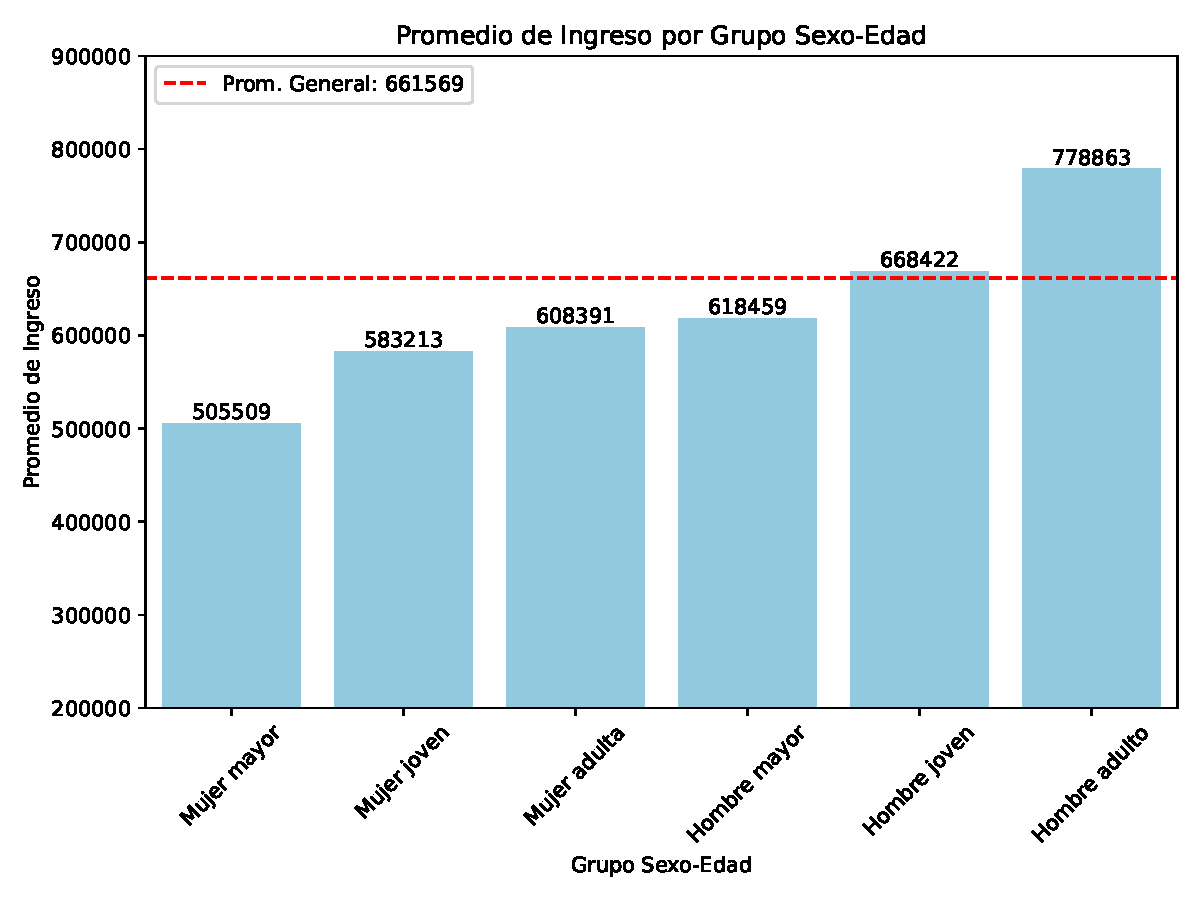
\includegraphics[width=\textwidth]{visualizaciones/preliminares/PromIngSexoEdad.pdf}
		\caption{Sexo y Edad}
		\label{1a}
	\end{subfigure}
	\hfill
	\begin{subfigure}[b]{0.49\textwidth}
		\centering
		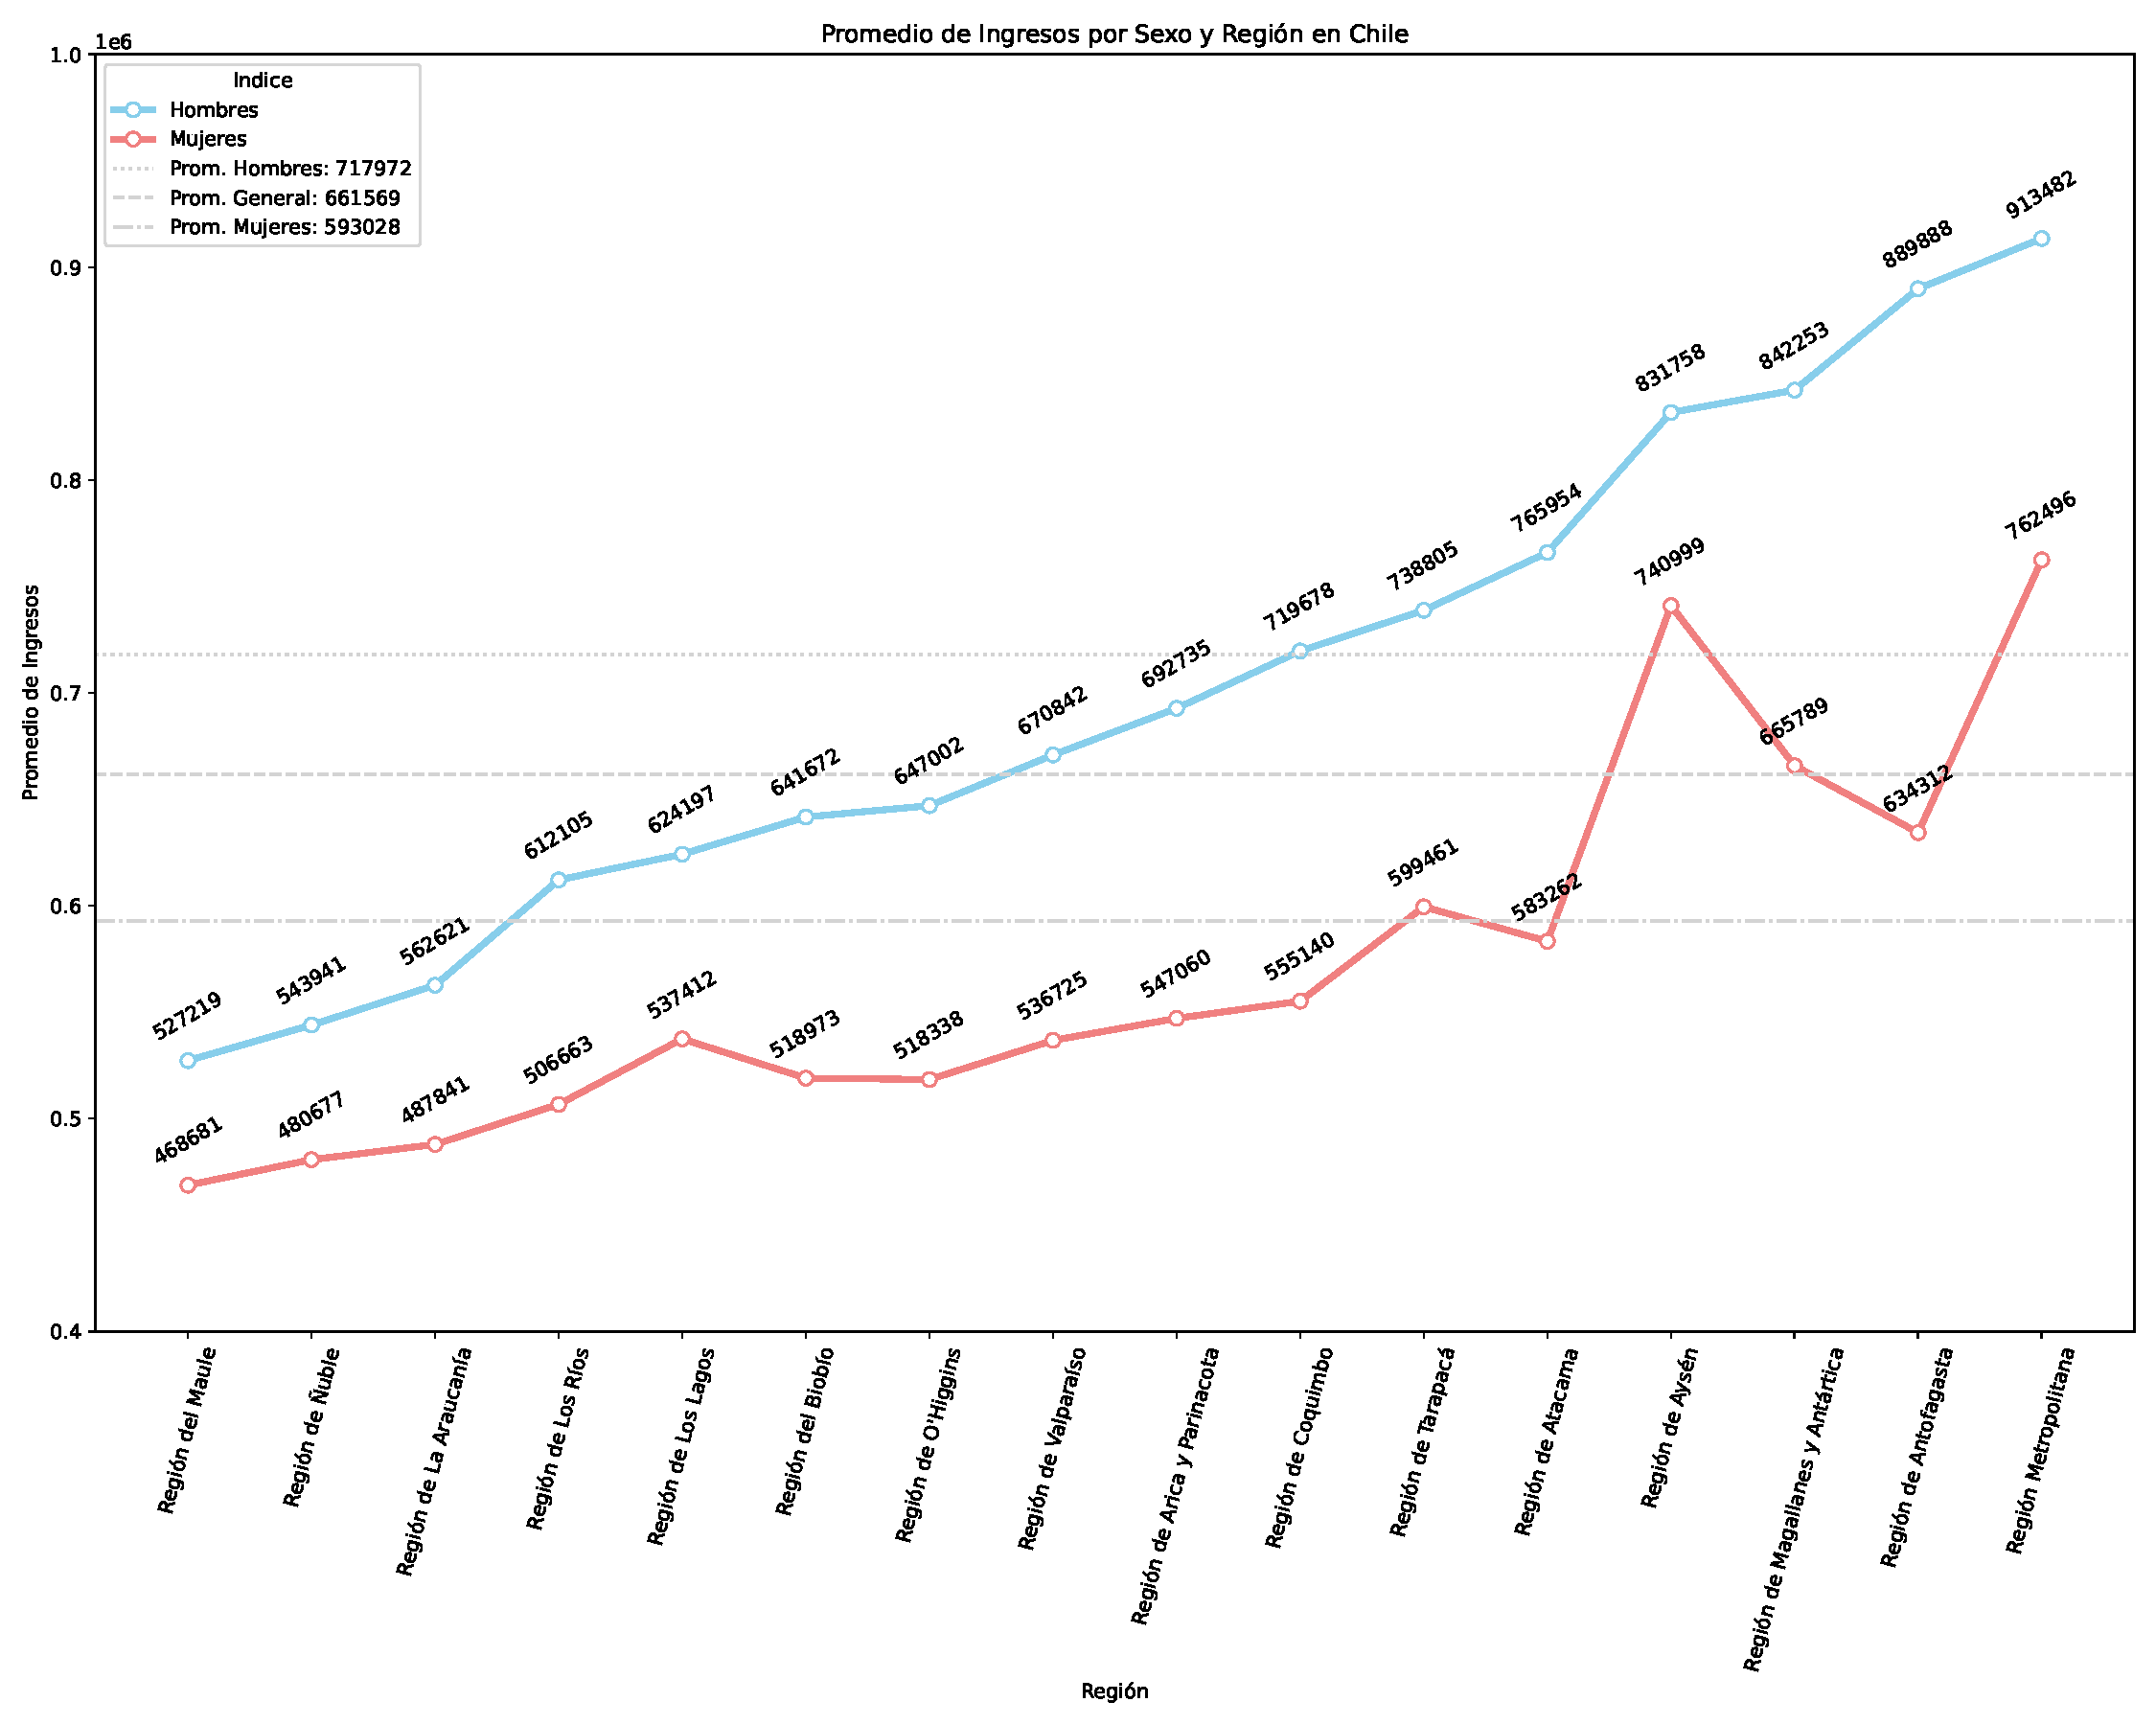
\includegraphics[width=\textwidth]{visualizaciones/preliminares/PromIngSexoRegion.pdf}
		\caption{Región}
		\label{1b}
	\end{subfigure}
	\caption{Representación preliminar de la Brecha Salarial de Género según Factores Sociodemográficos (1)\\Fuente: Elaboración propia en base a CASEN 2022. \citep{Proyecto1}}
	\label{01fig}
\end{figure}


\FloatBarrier

\begin{figure}[htbp]
	\centering
	\begin{subfigure}[b]{0.49\textwidth}
		\centering
		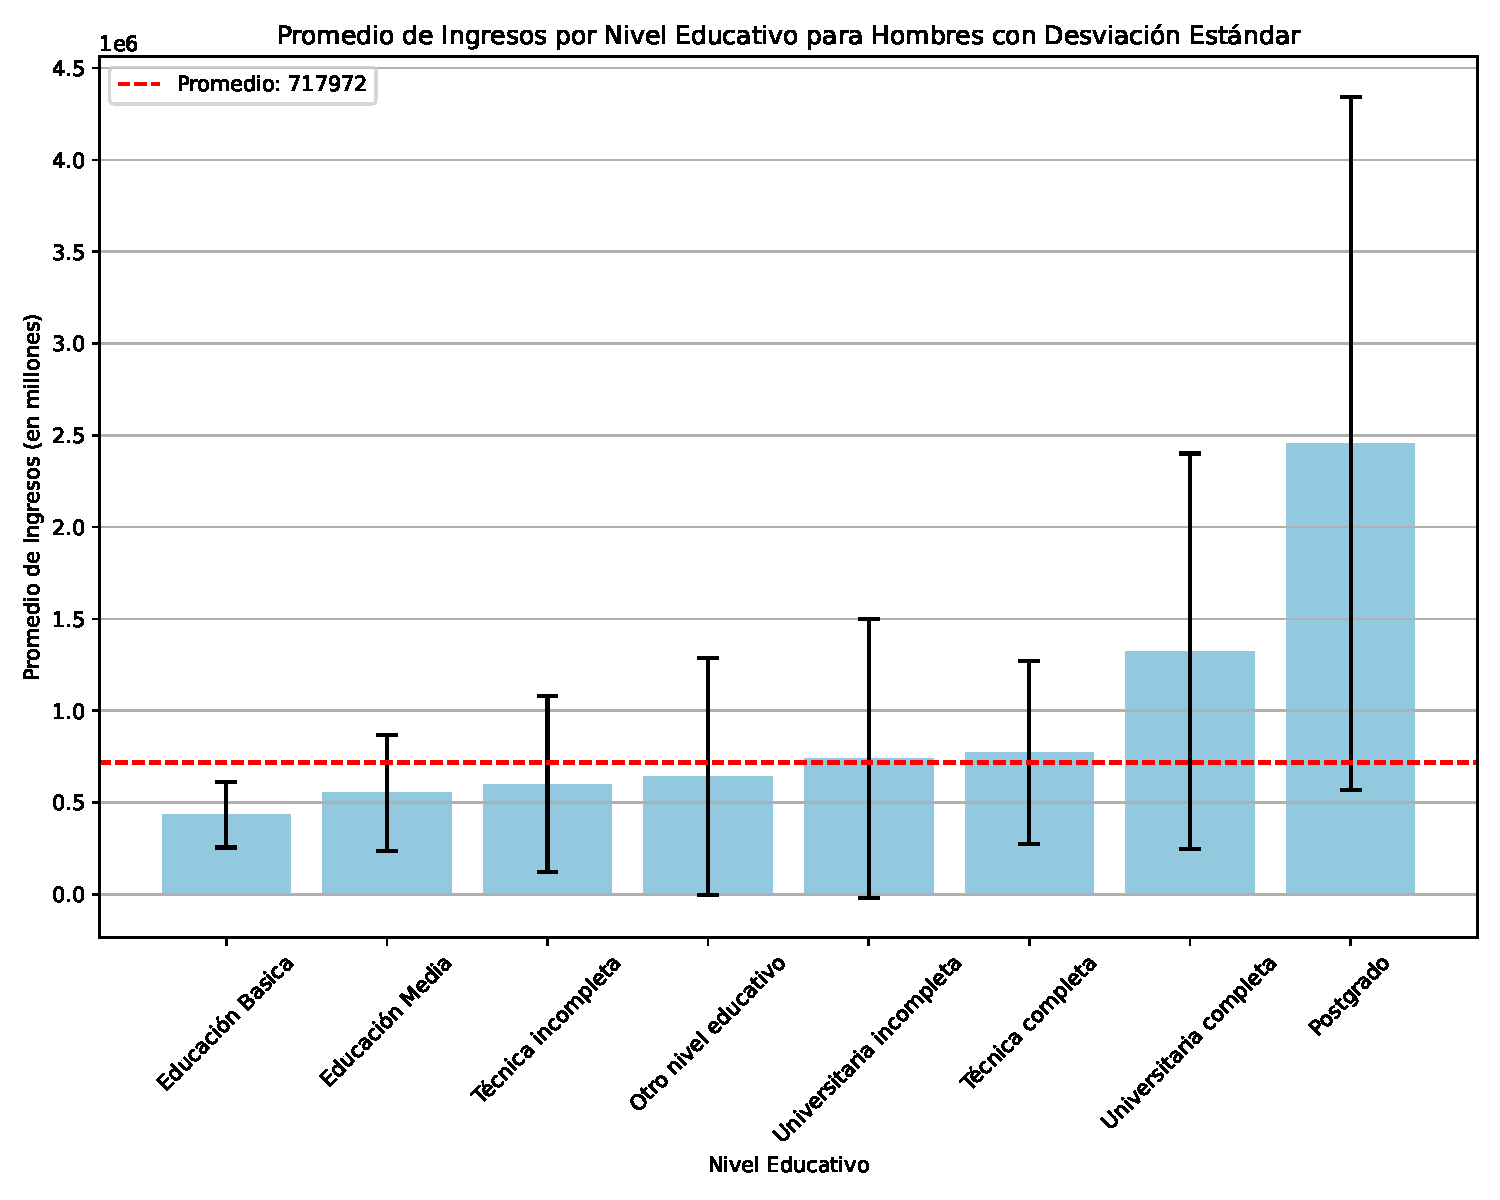
\includegraphics[width=\textwidth]{visualizaciones/preliminares/PromIngH_EducaDE.pdf}
		\caption{Hombres}
		\label{2a} 
	\end{subfigure}
	\hfill
	\begin{subfigure}[b]{0.49\textwidth}
		\centering
		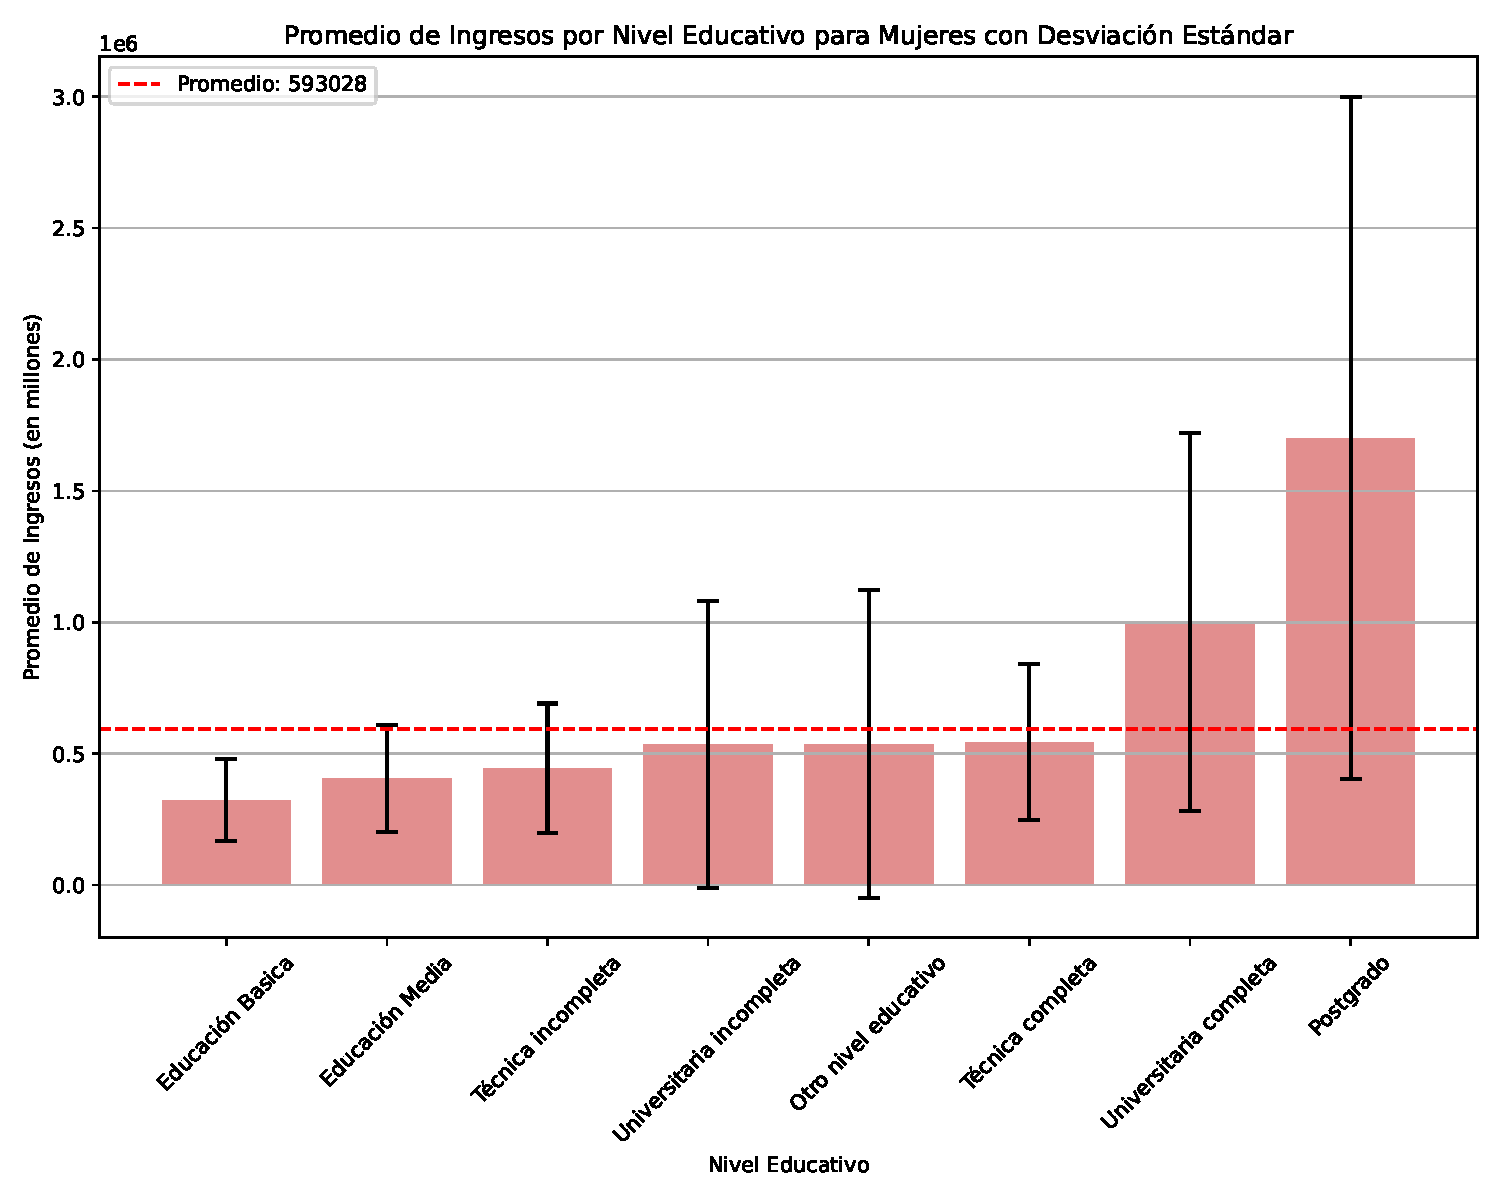
\includegraphics[width=\textwidth]{visualizaciones/preliminares/PromIngM_EducaDE.pdf}
		\caption{Mujeres}
		\label{2b}
	\end{subfigure}
	\caption{Representación preliminar de la Brecha Salarial de Género según Factores Sociodemográficos (2)\\Fuente: Elaboración propia en base a CASEN 2022. \citep{Proyecto1}}
	\label{02fig}
\end{figure}

\FloatBarrier

Como se logra apreciar en las figuras \ref{1a}, \ref{1b}, \ref{2a} y \ref{2b}, existe una notable desigualdad salarial entre hombres y mujeres. En todos los casos, el sueldo de las mujeres es inferior al de los hombres tanto en igual tramo etario, como en región y nivel educacional. Asimismo, se presenta una diferencia en la media salarial de \textdollar124.944. 

Estas observaciones, provenientes del análisis previo, plantean interrogantes sobre los factores de esta desigualdad. Ahora, se busca ampliar y profundizar en esta brecha para comprender mejor sus causas y características. El proyecto anterior está disponible en el siguiente \href{https://github.com/ElK1000o/Taller-Ciencia-de-Datos-I/tree/main/Proyecto}{repositorio de GitHub}.

Abordar esta problemática y promover que no siga sucediendo es crucial para avanzar hacia una sociedad más justa, equitativa y con igualdad de oportunidades. La brecha salarial de género no refleja únicamente las desigualdades del ámbito laboral, sino que genera también repercusiones en casi todos los índices de desigualdad. Según \citet{Castro-Romero2024}, el mercado laboral no solo presenta un imperativo ético, sino que también actúa como un catalizador para el crecimiento económico sostenible, la innovación y la cohesión social. Además, \citet{Cuellar2022}, destacan en su estudio que la brecha salarial de género se sitúa en un 29,6\%, revelando problemas estructurales en el mercado laboral. A pesar de que el mercado formal valora más a las mujeres desde 2001, la brecha salarial ha permanecido significativa por más de 30 años, confirmando la existencia de discriminación y sesgo de selección.

% \begin{center}
	%     \begin{minipage}{400px}
		%         Para cita en bloque
		%     \end{minipage}
	% \end{center}

A pesar de los años, esta desigualdad es persistente y cada vez más evidente. Se plantea que la base de la brecha de género es producto de que los hombres participan de posiciones sectoriales y ocupacionales mejor pagadas. Sin embargo, según \citet[pp. 333]{Ibanez2022}, ``eso no significa que la brecha desapareciera con la mera entrada de mujeres en sectores y ocupaciones masculinizadas (...) las ocupaciones feminizadas tienen más probabilidad de sufrir devaluación salarial que las masculinizadas''. Apoyando dicho punto y según explica \citet{Villar2010}, en un estudio realizado en España, se evidencia que los complementos salariales de los hombres son entre un 27 y un 30\% superiores a los que reciben las mujeres, incluso estando en la misma ocupación, empresa y con iguales características observables de capital humano.

Considerando lo anterior, esta investigación se basará en datos de la encuesta de Caracterización Socioeconómica Nacional (CASEN) y la Encuesta Nacional de Empleo (ENE), ambas de 2022 \citep{CASEN2022, ENE2022}. Estas encuestas servirán como un apoyo fundamental para verificar la brecha salarial en circunstancias de trabajo similares o iguales, así como para evaluar los posibles factores que promueven esta disparidad en diferentes áreas y posiciones laborales. El presente proyecto se encuentra disponible en \href{https://github.com/ElK1000o/Taller-Ciencia-de-Datos-II/tree/main/Proyecto}{GitHub} para su revisión y transparencia.

\section{Objetivos}

% En esta parte se debe escribir el objetivo general y los objetivos específicos del tema a desarrollar.

Teniendo en consideración los antecedentes que motivan esta investigación, surge la siguiente interrogante: ¿En qué medida las diferencias salariales entre hombres y mujeres en Chile pueden explicarse por factores laborales y no por el género en sí?

Para dar respuesta a esta pregunta y orientar la investigación, se han establecido los siguientes objetivos e hipótesis.

\subsection{Objetivo General}

% Se debe declarar el objetivo general de todo el proyecto de manera que contenga de manera global a todos los objetivos específicos.

El objetivo general de esta investigación consiste en evaluar la relación entre las diferencias salariales de género y las condiciones laborales en Chile, determinando si existen factores laborales que expliquen la brecha salarial, independientemente de si estas condiciones son similares o diferentes entre géneros.

\subsection{Objetivos Específicos}

% Los objetivos específicos se deben desprender lógicamente desde el objetivo general, y corresponde a tareas específicas que conllevan a resolver el objetivo del proyecto.

Para lograr lo anterior, considero apropiados los siguientes objetivos específicos:

\begin{itemize}
	\item Identificar las variables laborales que causen mayor impacto en los salarios en hombres y mujeres bajo condiciones similares.
	\item Comparar los ingresos de hombres y mujeres en diferentes condiciones sociodemográficas, ocupaciones,  contratos laborales, tipo de industria o sector, tipos de jornada y demás factores laborales.
	\item Evaluar si el género sigue siendo determinante en las diferencias salariales una vez controlados los factores laborales.
\end{itemize}

\section{Hipótesis de Investigación}

La hipótesis central de esta investigación es que, en promedio, las mujeres en Chile reciben salarios inferiores a los hombres incluso cuando se encuentran en similitud de condiciones laborales.

\section{Metodología} 

% En la parte de metodología se deben explicar las herramientas técnicas, modelos matemáticos, análisis estadísticos que se utilizarán para resolver el problema, detallando:

%    Breve introducción a los modelos matemáticos, estadísticos o algorítmicos que se utilizarán.
%    Definición de variables, datos o modelos a utilizar.
%    Todas las referencias necesarias para fundamentar y sustentar teóricamente.

Para llevar a cabo esta investigación, se empleará una metodología basada en herramientas de programación y análisis de datos. Se elige Python, un lenguaje ampliamente utilizado en la ciencia de datos, acompañado de las siguientes librerías:

\begin{itemize}
	\item \textbf{pandas}: Para la manipulación y análisis de datos, permitiendo realizar operaciones como filtrado, agrupamiento y transformación de datos.
	\item \textbf{numpy}: Para diversos cálculos numéricos y operaciones matemáticas.
	\item \textbf{matplotlib y seaborn}: Empleadas para la visualización de los datos obtenidos, descubrimiento de insights y facilitación en la interpretación de resultados.
	\item \textbf{scikit-learn}: Para implementación de modelos de clasificación utilizando RandomForestClassifier.
\end{itemize}

Los datos de las encuestas CASEN y ENE fueron obtenidos desde el sitio web del \href{https://observatorio.ministeriodesarrollosocial.gob.cl/encuesta-casen-2022}{Observatorio Social} y del \href{https://www.ine.gob.cl/estadisticas/sociales/mercado-laboral/ocupacion-y-desocupacion}{INE}, respectivamente. Ambos conjuntos de datos fueron procesados en Python utilizando las librerías mencionadas anteriormente. Para facilitar la comprensión de las encuestas y el significado de sus variables se recurrió a los respectivos libros de código y cuestionarios correspondientes, permitiendo y agilizando la realización de distintas recodificaciones, asignación de valores nulos, creación de nuevas variables y el filtrado de los datos según las necesidades del análisis. 

Para complementar el análisis de los datos obtenidos de las encuestas CASEN y ENE, se recurrirá al uso de estadísticos descriptivos que permitirán resumir y entender mejor las características de la muestra. Los que se utilizarán principalmente en el proyecto son:

\begin{itemize}
	\item \textbf{Medidas de tendencia central (MTC)}: Se calcularán la media, mediana y moda en distintas variables como edad, ingreso, horas/días trabajados, etc.
	\item \textbf{Desviación estándar}: Para medir la dispersión o variabilidad de los factores mencionados.
	\item \textbf{Porcentajes y proporciones}: Se realizarán tablas de contigencia con la finalidad de comparar la distribución de las variables sociodemográficas y laborales en hombres y mujeres, facilitando la identificación de posibles sesgos o desigualdades, lo que permitiría encontrar factores clave que puedan explicar la brecha salarial.
	\item \textbf{Correlación de Spearman}: Se analizará la correlación de todos los factores presentes con la finalidad de buscar y/o hallar patrones que permitan dar respuesta a la incógnita planteada.
\end{itemize}

Las técnicas estadísticas declaradas anteriormente proporcionarán una base sólida para una buena exploración, permitiendo una comparación clara y estructurada de las variables clave involucradas en la brecha salarial. Además, para su mejor visualización, los resultados obtenidos irán generalmente acompañados de gráficas (como gráficos de barra, dispersión, histogramas, etc.) y tablas que sean representativas de los datos.

Respecto a la selección de variables, se consideraron factores sociodemográficos y laborales clave, como lo son: sexo, edad, nivel educativo, región de residencia, sueldo/ingreso, tipo de contrato, temporada de trabajo, jornada laboral, horas trabajadas diarias/semanales, días trabajados semanalmente, grupo ocupacional, actividad actual, razones de no actividad y rol laboral.

En cuanto a revisión de literatura, se realizó una búsqueda a través del Sistema de Bibliotecas de la Universidad Mayor (SIBUM), recopilando artículos y libros desde diversas plataformas, tales como ``elibro'', ``Web of Science (WoS)'' y ``EBSCO'', sumado a literatura obtenida de otros sitios de búsqueda como ``Google Académico'' y ``SciELO''. Los parámetros de búsqueda se centraron en términos relacionados con el tema a investigar, empleando las siguientes palabras clave: ``Salarial'', ``Género'', ``Brecha'', ``Gender gap'' y ``Wages''. 

\section{Modelo computacional y algoritmo}

El modelo computacional y algoritmo utilizado en este proyecto se implementó a través de Python con sus respectivas librerías, se utilizó la librería pandas para diversas recodificaciones y creación de nuevas variables, como por ejemplo, la variable ``BuscarTrabajo'' en la ENE 2022 se creó en base a ``e3\_1'', ``e3\_2'', ``e3\_3'', ``e3\_4'', ``e3\_5'', ``e3\_6'', ``e3\_7'', ``e3\_8'', ``e3\_9'', ``e3\_10'' y ``e3\_11'' (11 variables). También se generó una nueva variable de edad por tramos en ambos conjuntos ENE y CASEN; variable ``sexo\_edad'' que contiene la anterior combinada con el sexo, entre otras.

Se utilizó la librería de numpy para diversos cálculos y las librerías matplotlib y seaborn para realizar los gráficos presentes en este informe. Por otro lado, el uso de la librería scikit-learn permitió implementar algoritmos de Machine Learning con los que se buscó clasificar el sexo en base a factores laborales contenidos en CASEN y ENE. El detalle de los modelos con RandomForestClassifier implementados en ambas encuestas se presenta a continuación:

\FloatBarrier

\begin{lstlisting}[style=mystyle, caption={Modelo RandomForestClassifier en CASEN 2022}, label={01py}]
	# Mejor modelo encontrado para CASEN 2022 (Accuracy 0.68)
		
	rf = RandomForestClassifier(n_estimators=32, # numero de arboles
								criterion="gini", # medida para evaluar
								max_depth=8, # profundidad
								n_jobs=-1,
								verbose=1,
								random_state=20230728)
\end{lstlisting}

\FloatBarrier

\begin{lstlisting}[style=mystyle, caption={Modelo RandomForestClassifier en ENE 2022}, label={02py}]
	# Mejor modelo encontrado para ENE 2022 (Accuracy 0.81)
		
	rf = RandomForestClassifier(n_estimators=54, # numero de arboles
								criterion="gini", # medida para evaluar
								max_depth=9, # 9 de profundidad
								n_jobs=-1,
								verbose=1,
								random_state=20230728)
\end{lstlisting}


\FloatBarrier

Respecto a los resultados obtenidos con el modelo del Listing \ref{01py} nos encontramos con lo siguiente: 

\FloatBarrier
\begin{figure}[htbp]
	\centering
	\begin{subfigure}[b]{0.49\textwidth}
		\centering
		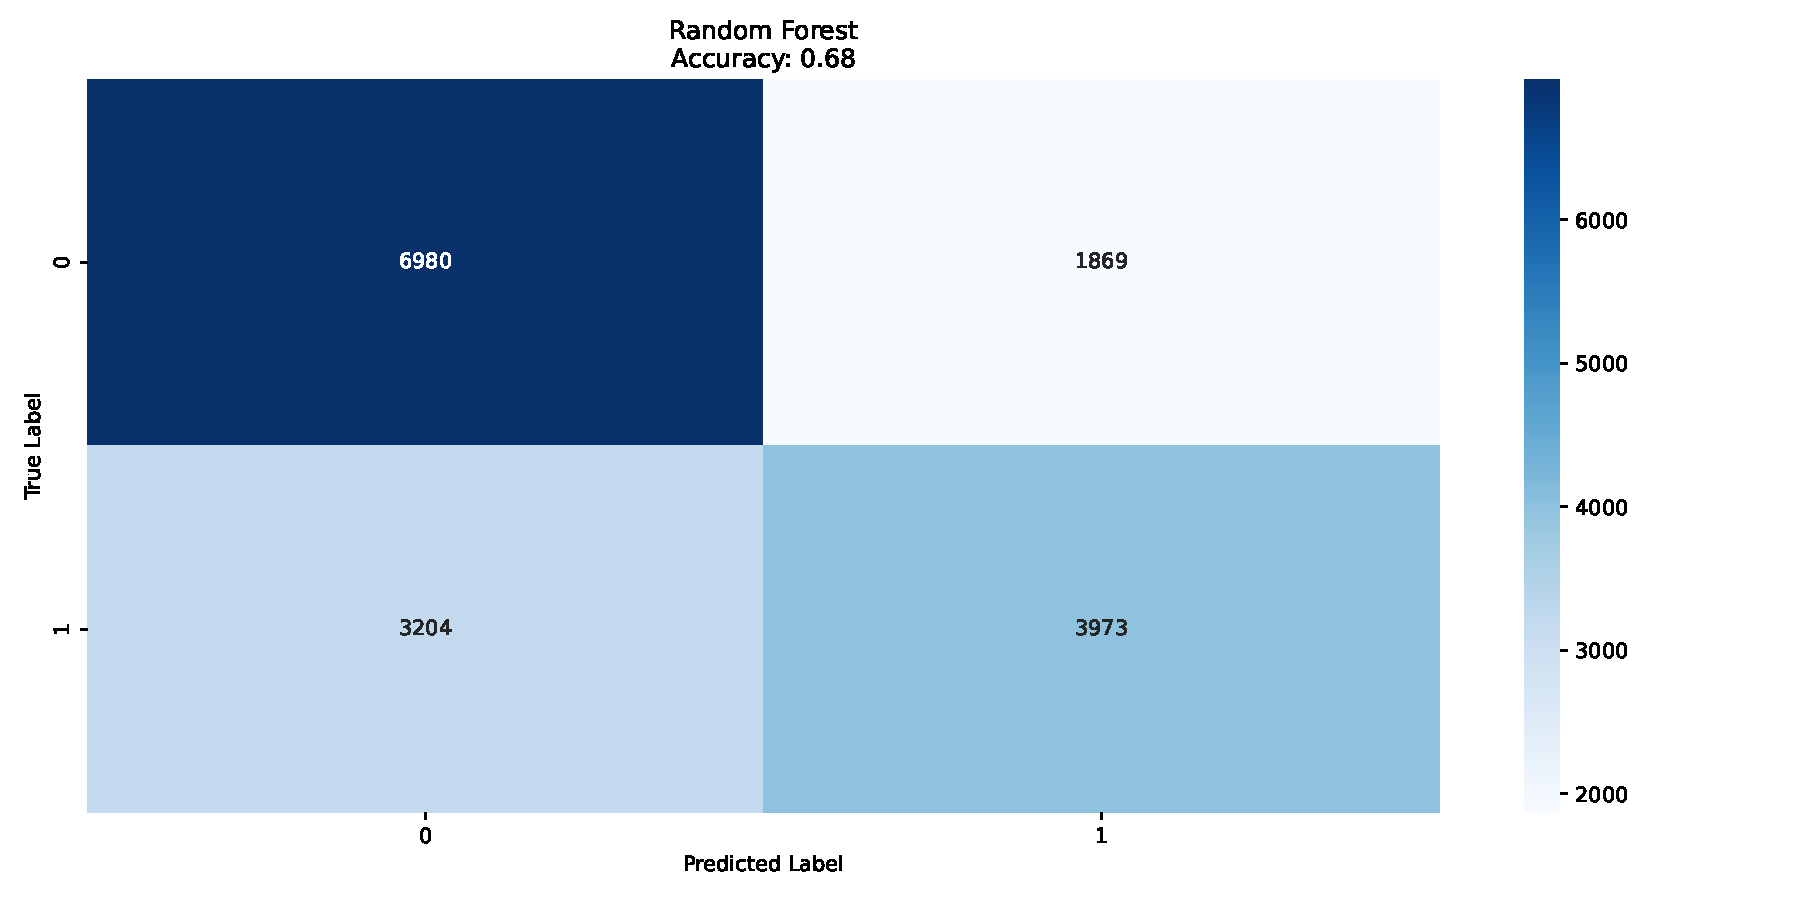
\includegraphics[width=\textwidth]{visualizaciones/finales/confusionCASEN2022.pdf}
		\caption{Matriz de Confusión Modelo Random Forest CASEN 2022.}
		\label{3a} 
	\end{subfigure}
	\hfill
	\begin{subfigure}[b]{0.49\textwidth}
		\centering
		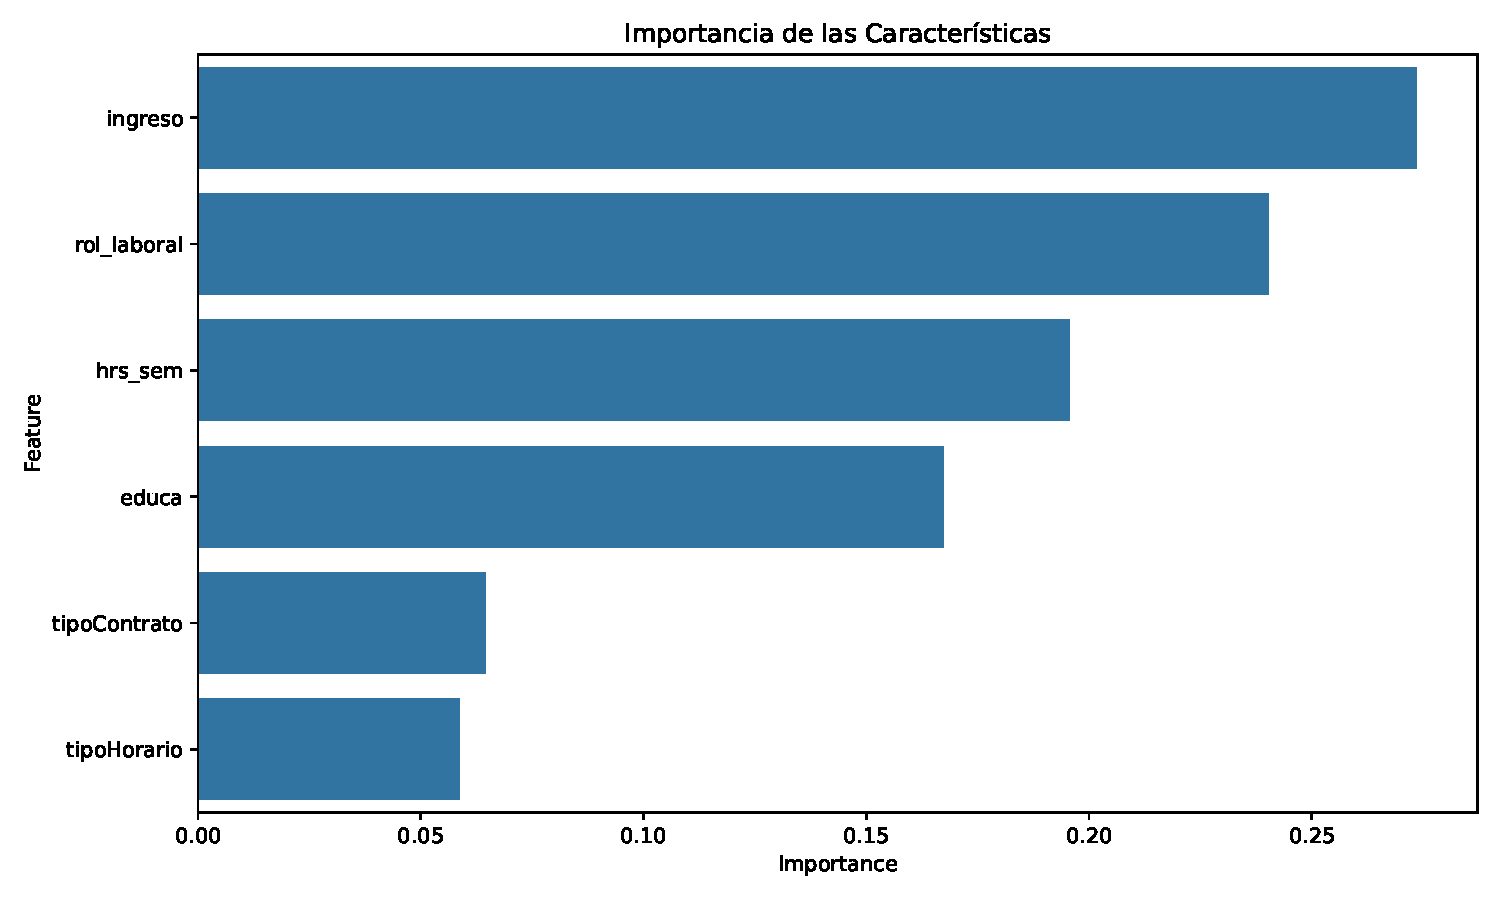
\includegraphics[width=\textwidth]{visualizaciones/finales/importanciasCASEN2022.pdf}
		\caption{Importancia de Factores Modelo Random Forest CASEN 2022.}
		\label{3b}
	\end{subfigure}
	\caption{Modelo conseguido CASEN 2022.}
	\label{03fig}
\end{figure}

\FloatBarrier

Como se observa en la Figura \ref{3a}, el modelo conseguido no alcanzó una precisión muy alta, obteniendo un \textit{accuracy} de 0.68 y logrando clasificar de mejor manera a los hombres (0) que a las mujeres (1). No obstante a lo anterior, la Figura \ref{3b} deja en evidencia que lo más importante dentro de las variables laborales de CASEN para lograr clasificar hombres y mujeres con mayor tasa de éxito es el ingreso, seguido del rol laboral y las horas semanales. 

Por otro lado, en cuanto a los resultados obtenidos con el modelo del Listing \ref{02py} se aprecia lo siguiente:

\FloatBarrier

\begin{figure}[htbp]
	\centering
	\begin{subfigure}[b]{0.49\textwidth}
		\centering
		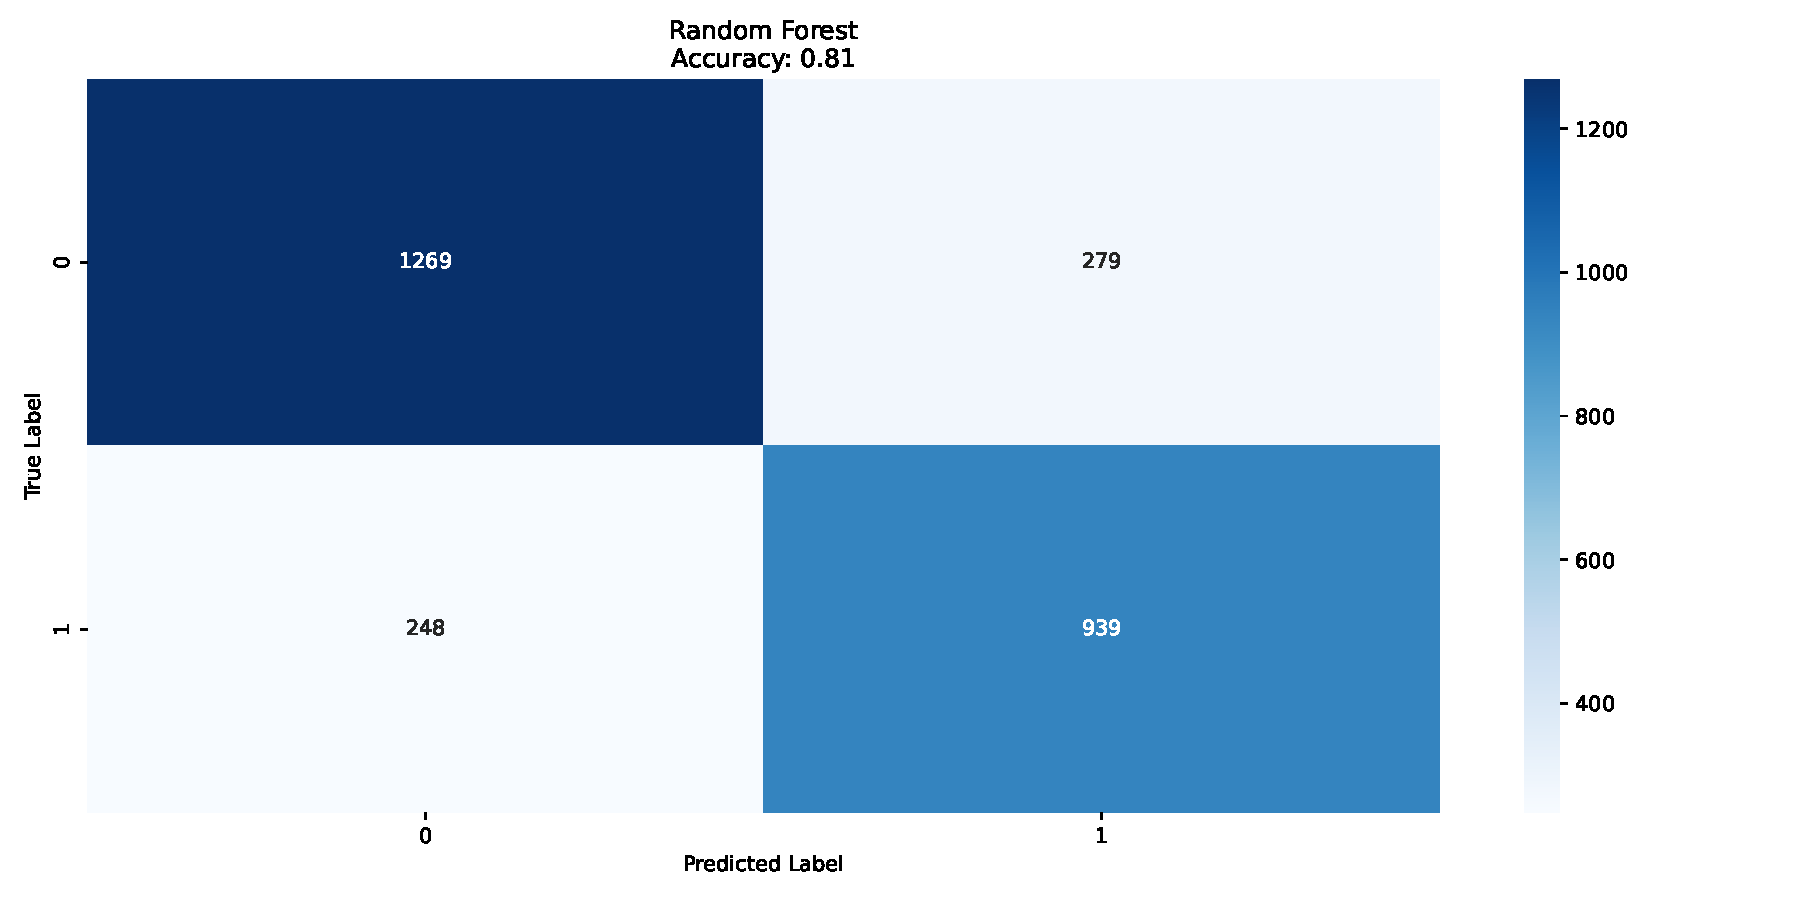
\includegraphics[width=\textwidth]{visualizaciones/finales/confusionENE2022.pdf}
		\caption{Matriz de Confusión Modelo Random Forest ENE 2022.}
		\label{4a} 
	\end{subfigure}
	\hfill
	\begin{subfigure}[b]{0.49\textwidth}
		\centering
		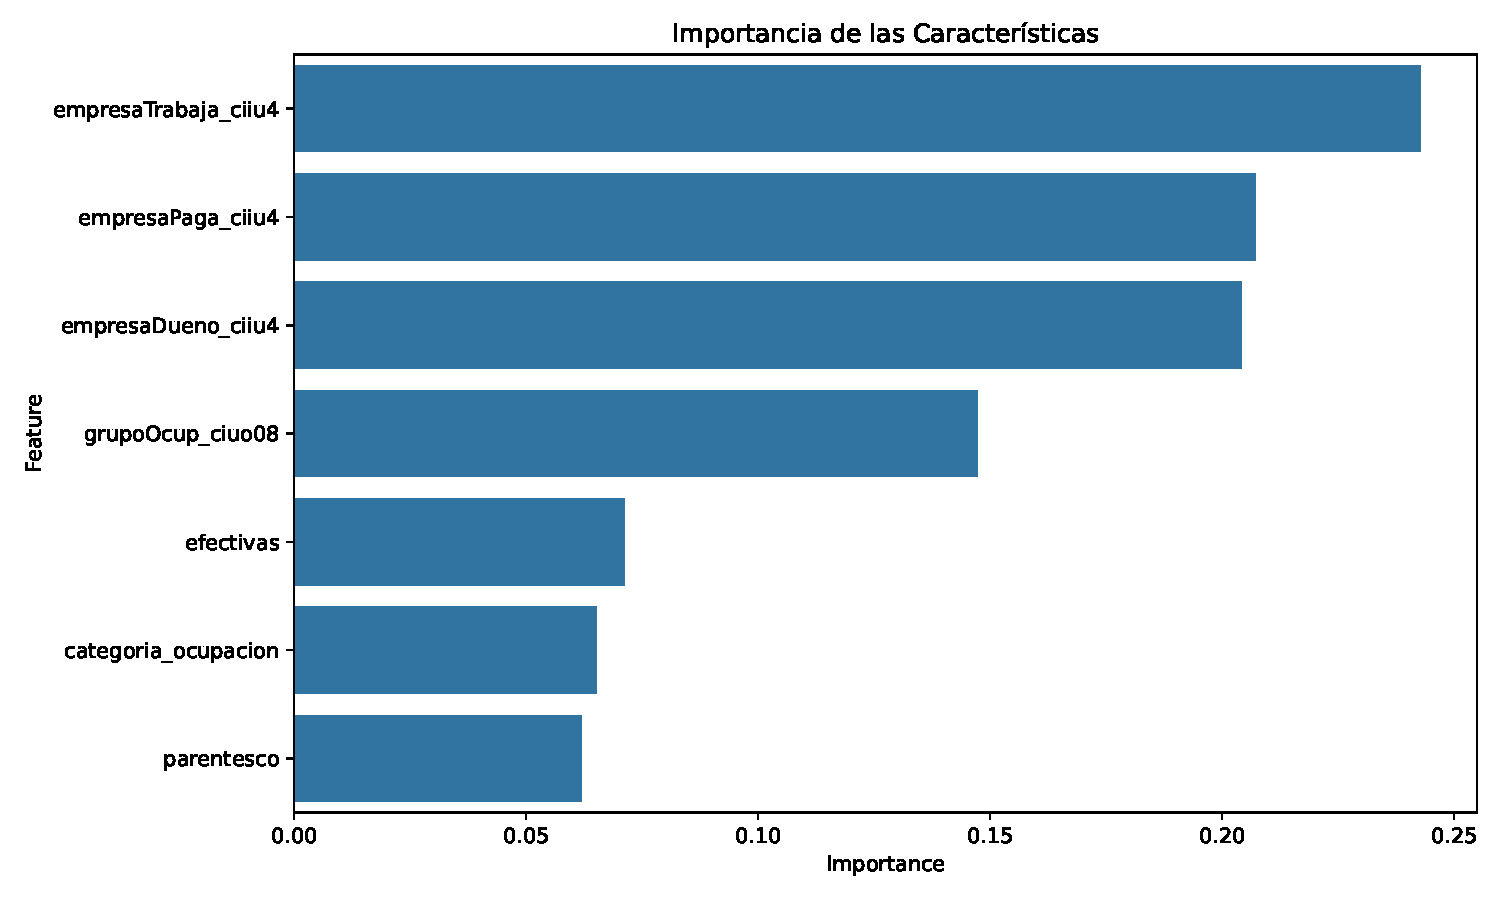
\includegraphics[width=\textwidth]{visualizaciones/finales/importanciasENE2022.pdf}
		\caption{Importancia de Factores Modelo Random Forest ENE 2022.}
		\label{4b}
	\end{subfigure}
	\caption{Modelo conseguido ENE 2022.}
	\label{04fig}
\end{figure}

\FloatBarrier

La Figura \ref{4a} presenta una considerable mejora en la clasificación de hombres y mujeres, obteniendo un \textit{accuracy} de 0.81, aunque se logra observar que sigue costando un poco más clasificar correctamente al género femenino. Para este caso, según muestra la Figura \ref{4b} las mejores variables para lograr la mayor precisión dentro de la clasificación son factores rama de actividad económica de la empresa en la que trabaja, paga o de la que se es dueño el encuestado según CIIU-4, así como el grupo ocupacional establecido según CIUO-08, lo que conjunto a lo visto en CASEN, podría dar lugar a la inferencia de que las áreas laborales y el ingreso son de los factores más decisivos en la clasificación. Es decir, la brecha podría ser explicada (en cierto porcentaje) por estas condiciones laborales.

\section{Resultados}

A continuación se detallarán los resultados obtenidos en este proyecto. 

\FloatBarrier

\begin{table}[htbp]
	\centering
	
	% Subtabla ENE 2022
	\begin{subtable}[ht]{\textwidth}
		\centering
		\resizebox{\textwidth}{!}{ 
			\begin{tabular}{|c|c|c|c|c|c|c|c|c|}
				\hline
				\multicolumn{1}{|c|}{} & \multicolumn{4}{|c|}{\textbf{Hombres}} & \multicolumn{4}{|c|}{\textbf{Mujeres}} \\
				\hline
				\textbf{} & \textbf{Edad} & \textbf{Horas/Semana} & \textbf{Horas/Día} & \textbf{Días/Semana} & \textbf{Edad} & \textbf{Horas/Semana} & \textbf{Horas/Día} & \textbf{Días/Semana} \\
				\hline
				\textbf{count} & 40306.00 & 40144.00 & 28138.00 & 36025.00 & 31846.00 & 31743.00 & 22959.00 & 30396.00 \\
				\textbf{mean} & 44.59 & 42.53 & 8.35 & 5.12 & 42.86 & 38.19 & 7.61 & 4.84 \\
				\textbf{std} & 14.52 & 12.67 & 1.97 & 1.12 & 13.35 & 14.82 & 2.41 & 1.29 \\
				\textbf{min} & 18.00 & 1.00 & 1.00 & 1.00 & 18.00 & 1.00 & 1.00 & 1.00 \\
				\textbf{25\%} & 32.00 & 40.00 & 8.00 & 5.00 & 32.00 & 30.00 & 6.00 & 5.00 \\
				\textbf{50\%} & 44.00 & 45.00 & 9.00 & 5.00 & 42.00 & 44.00 & 8.00 & 5.00 \\
				\textbf{75\%} & 56.00 & 45.00 & 9.00 & 6.00 & 53.00 & 45.00 & 9.00 & 5.00 \\
				\textbf{max} & 95.00 & 148.00 & 24.00 & 7.00 & 94.00 & 140.00 & 24.00 & 7.00 \\
				\hline
			\end{tabular}
		}
		\caption{Estadísticas descriptivas para ENE 2022.}
	\end{subtable}
	
	\vspace{0.5cm} % Espaciado entre subtables
	
	% Subtabla CASEN 2022
	\begin{subtable}[ht]{\textwidth}
		\centering
		\resizebox{\textwidth}{!}{
			\begin{tabular}{|c|c|c|c|c|c|c|} 
				\hline
				\multicolumn{1}{|c|}{} & \multicolumn{3}{c|}{\textbf{Hombres}} & \multicolumn{3}{c|}{\textbf{Mujeres}} \\
				\hline
				\textbf{} & \textbf{Edad} & \textbf{Horas/Semana} & \textbf{Ingreso} & \textbf{Edad} & \textbf{Horas/Semana} & \textbf{Ingreso} \\
				\hline
				\textbf{count} & 32719.00 & 32445.00 & 32719.00 & 26925.00 & 26817.00 & 26925.00 \\
				\textbf{mean} & 42.33 & 44.82 & 717972.47 & 41.16 & 40.89 & 593028.20 \\
				\textbf{std} & 13.88 & 9.42 & 708492.08 & 12.68 & 10.53 & 552483.67 \\
				\textbf{min} & 18.00 & 1.00 & 0.00 & 18.00 & 1.00 & 0.00 \\
				\textbf{25\%} & 31.00 & 45.00 & 400000.00 & 31.00 & 40.00 & 350000.00 \\
				\textbf{50\%} & 41.00 & 45.00 & 500000.00 & 40.00 & 45.00 & 440000.00 \\
				\textbf{75\%} & 54.00 & 45.00 & 800000.00 & 51.00 & 45.00 & 670000.00 \\
				\textbf{max} & 90.00 & 105.00 & 25000000.00 & 92.00 & 84.00 & 12000000.00 \\
				\hline
			\end{tabular}
		}
		\caption{Estadísticas descriptivas para CASEN 2022.}
	\end{subtable}
	
	\caption{Estadísticas descriptivas para hombres y mujeres.}
	\label{tab:estadisticas_descriptivas}
	
\end{table}

\FloatBarrier

Las tablas en el Cuadro \ref{tab:estadisticas_descriptivas} presentan distintas mediciones de variables, por un lado se evidencia que las distribuciones etarias son bastante similares en ambas encuestas para hombres y mujeres, por lo que podemos realizar una buena comparación del resto de variables laborales entre ENE y CASEN. 

Por un lado, se muestra que en la variable compartida (horas/semana) las mujeres trabajan menos horas semanalmente que los hombres en promedio, con una diferencia de aproximadamente 4 horas, sumado a que posee mayor variabilidad en sus datos, ya que su desviación estándar es un poco mayor a la de los hombres, en ambos casos. Coinciden en horas para el segundo y tercer cuartil en las dos encuestas (45 horas semanales), con una ligera disparidad en la ENE (1 hora). Sin embargo, la diferencia más notoria es en el primer cuartil, donde tenemos 5 horas de contraste en CASEN y 10 horas en la ENE, indicando menos horas laborales para las mujeres. En cuanto a horas diarias y días a la semana, las mujeres se encuentran levemente por debajo en comparación con los hombres. Sin embargo en ningún caso son cifras muy alarmantes.

Por parte del ingreso recibido mensualmente. Podemos observar que en todas las mediciones (exceptuando el mínimo) las mujeres reciben un salario inferior a los hombres que no parece ser proporcional con las discrepancias detectadas en horas y días de trabajo y mucho menos edad.

\FloatBarrier

\begin{figure}[htbp]
	\centering
	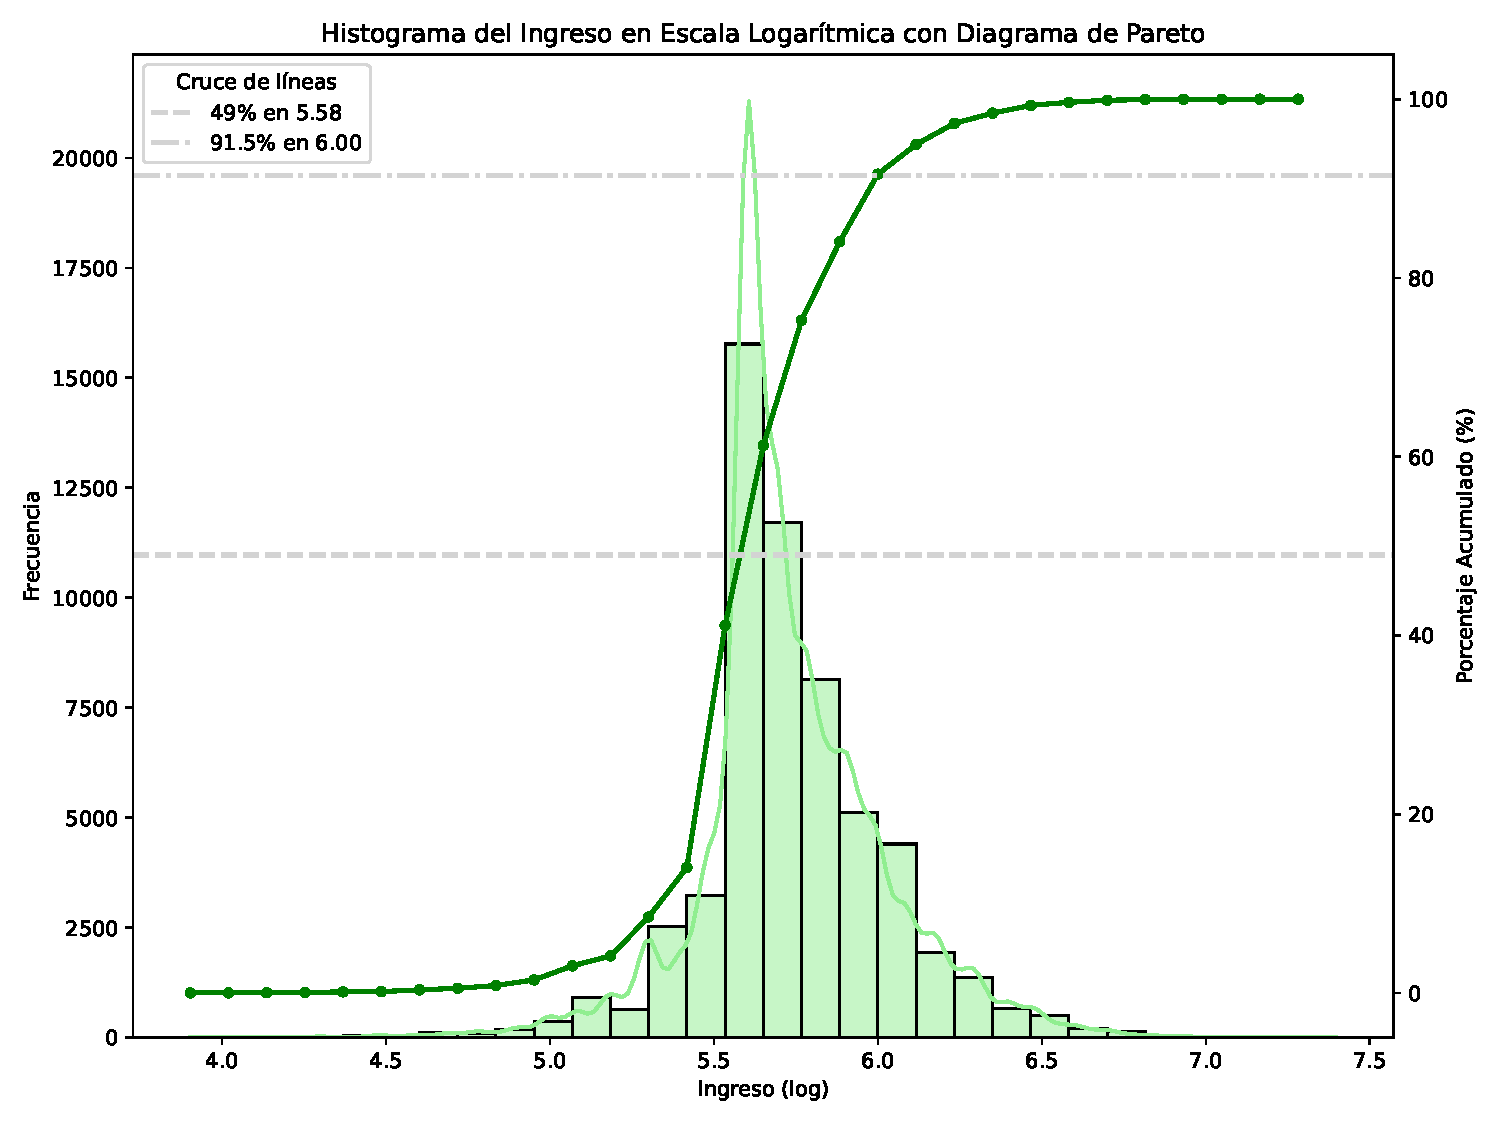
\includegraphics[width=0.65\textwidth]{visualizaciones/finales/Histo_ing_CASEN2022.pdf}
	\caption{Histograma Ingreso General (Escala logarítmica + Pareto). Elaborado en base a CASEN 2022.}
	\label{05fig} 
\end{figure}

\FloatBarrier	

\begin{table}[htbp]
	\centering
	\begin{tabularx}{\textwidth}{|X|X|X|}
		\hline
		Fecha de Cambio & 18 a 65 años & Ley y Fecha de Promulgación\\
		\hline
		01-ene-2022 & 350.000 & 21.360 (05-07-2021) \\\hline
		01-may-2022 & 380.000 & 21.456 (26-05-2022) \\\hline
		01-ago-2022 & 400.000 & 21.456 (26-05-2022) \\\hline
	\end{tabularx}
	\caption{\label{sueldominimo} Sueldo mínimo 2022. \citep{cyma}}
\end{table}

\FloatBarrier

El histograma de la Figura \ref{05fig} muestra la variable ingreso conjunta de hombres y mujeres en escala logarítmica (\(\log_{10}\)). Siguiendo la información entregada por el Cuadro \ref{sueldominimo} vemos que el sueldo mínimo fluctuó entre \textdollar350.000 y \textdollar400.000, si se asume \textdollar380.000 como sueldo promedio para todo el año, tenemos que en escala logarítmica un 49\% de la población cuenta con un sueldo mínimo o menos y alrededor del 91.5\% recibe un ingreso menor o igual a \textdollar1.000.000. No obstante, es pertinente para este proyecto realizar una comparativa de este mismo histograma para cada género.

\FloatBarrier

\begin{figure}[htbp]
	\centering
	\begin{subfigure}[b]{0.49\textwidth}
		\centering
		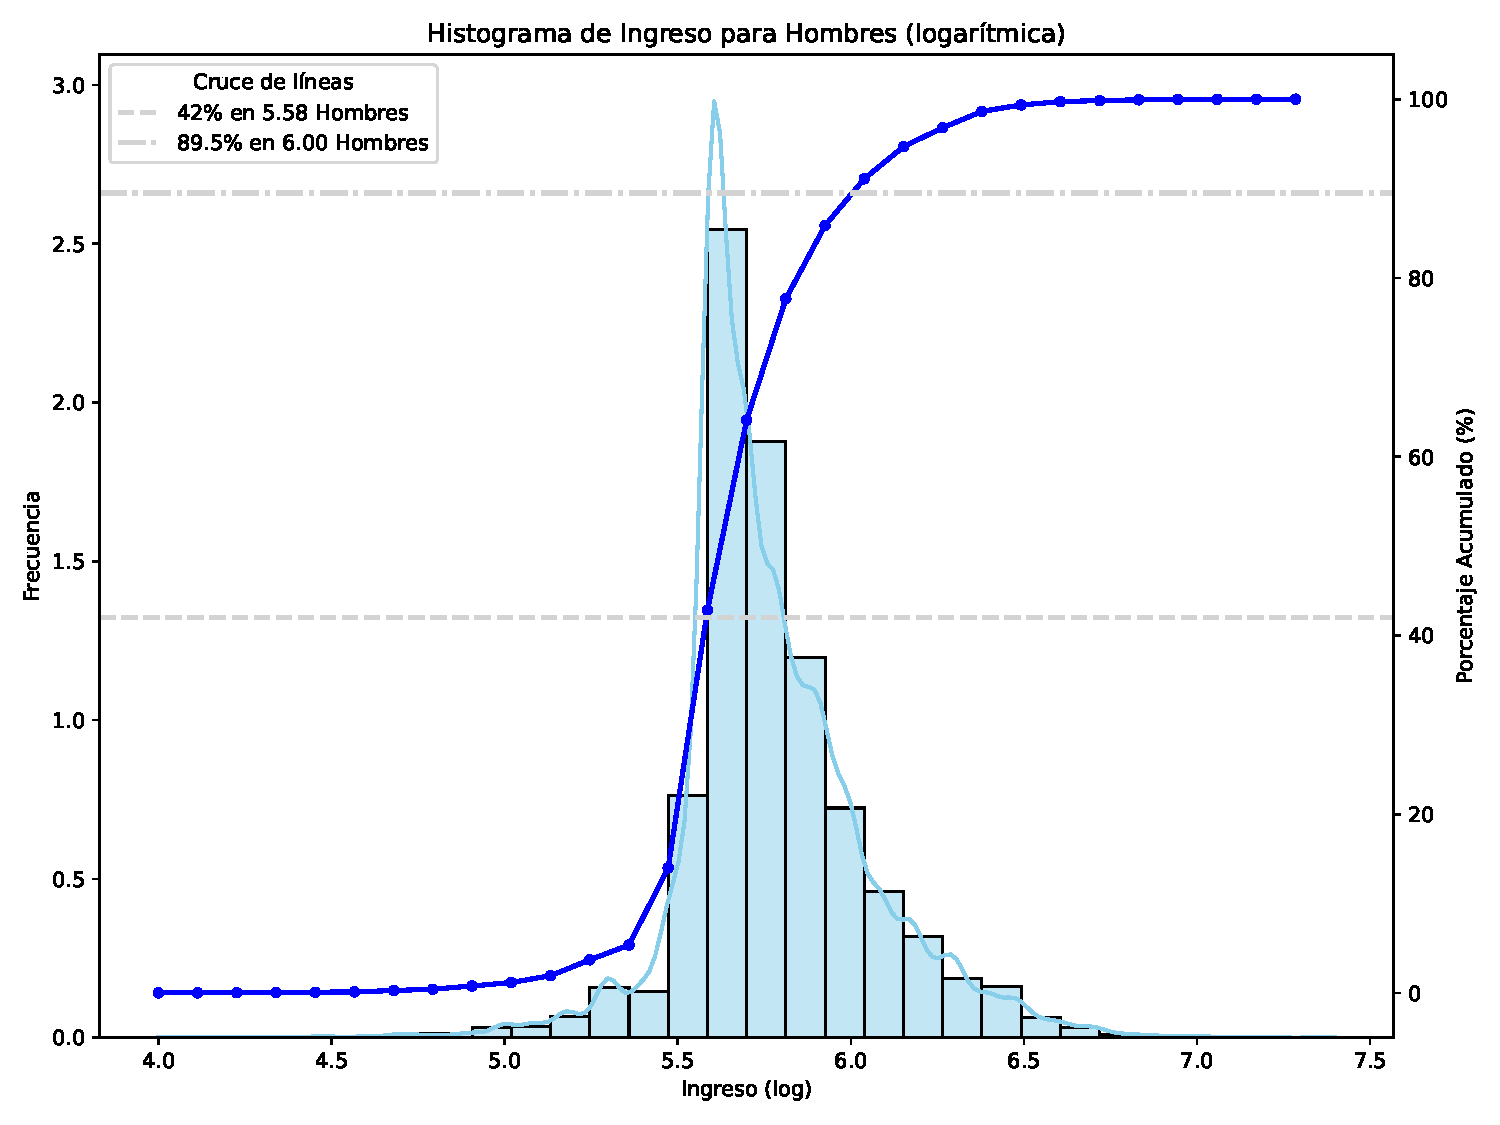
\includegraphics[width=\textwidth]{visualizaciones/finales/Histo_ing_h_CASEN2022.pdf}
		\caption{Histograma Hombres.}
		\label{6a} 
	\end{subfigure}
	\hfill
	\begin{subfigure}[b]{0.49\textwidth}
		\centering
		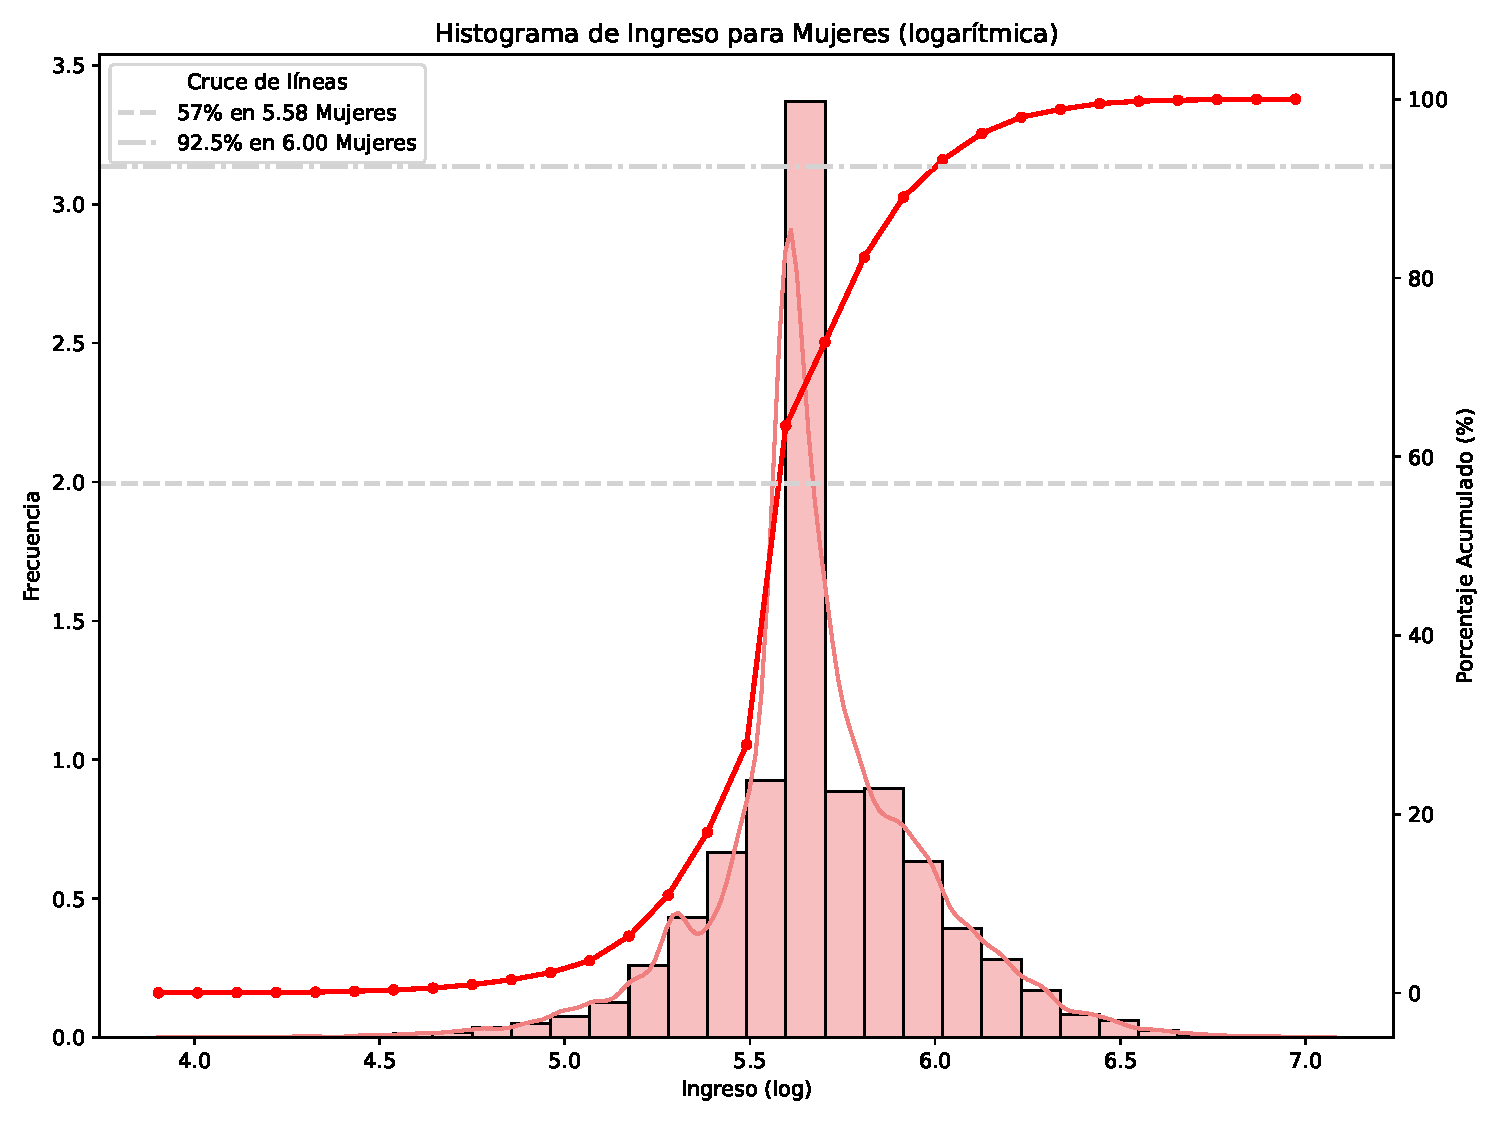
\includegraphics[width=\textwidth]{visualizaciones/finales/Histo_ing_m_CASEN2022.pdf}
		\caption{Histograma Mujeres.}
		\label{6b}
	\end{subfigure}
	\caption{Histogramas separados de ingreso para Hombres y Mujeres. Elaborado en base a CASEN 2022.}
	\label{06fig}
\end{figure}

\FloatBarrier

Desde esta perspectiva vemos nuevamente la brecha salarial de género existente. Es menor el porcentaje de los hombres que recibe un sueldo igual o inferior al mínimo, un 42\% comparando con el 57\% de las mujeres, lo cual es una diferencia notable. Por otro lado, en sueldos iguales o inferiores a \textdollar1.000.000 también es menor este porcentaje, presentando un 3\% de diferencia con 89.5 y 92.5\% respectivamente. Observamos también una gran concentración de mujeres en la posición correspondiente de $10^{5.6}$ a $10^{5.7}$ aproximadamente, es decir, la mayoría de ellas se encuentra en un rango entre \textdollar398.000 y \textdollar501.000, mientras que los hombres tienden en su distribución a estar más concentrados en las zonas de salarios más altos. 

Lo anterior, nuevamente no hace sentido, si bien se observan diferencias en cuanto a horas y días trabajados semanalmente, estas discrepancias en el sueldo no son proporcionales.

\FloatBarrier

\begin{figure}[htbp]
	\centering
	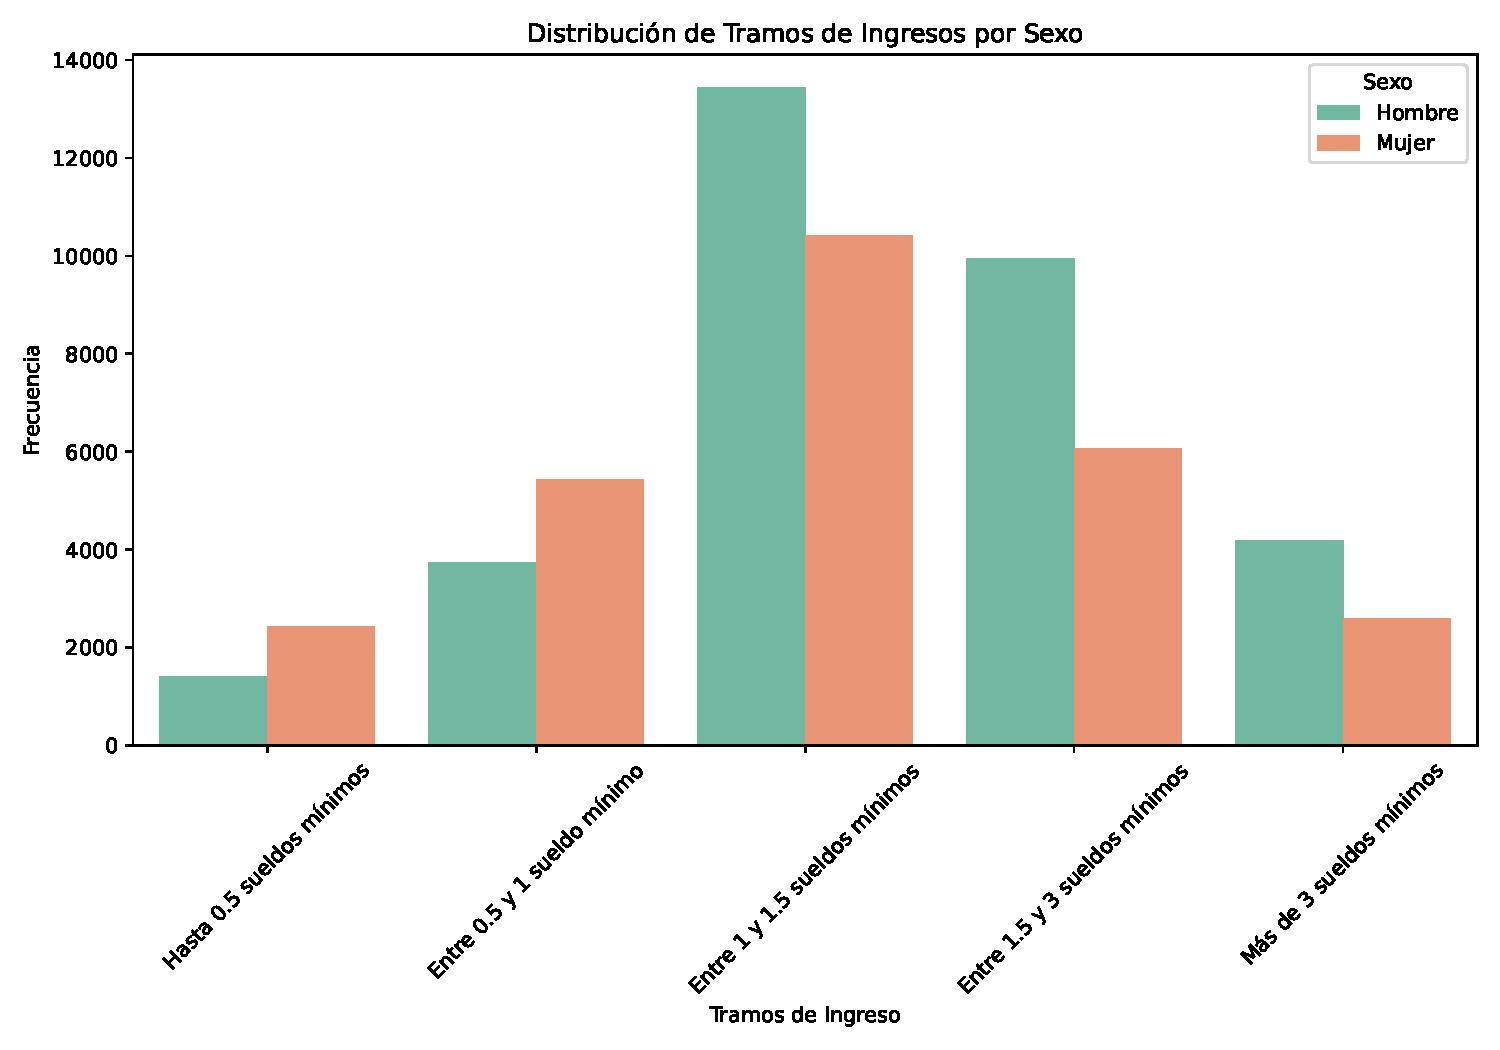
\includegraphics[width=0.65\textwidth]{visualizaciones/finales/TramoIngreso_SexoCASEN2022.pdf}
	\caption{Distribución en los diferentes tramos de ingreso por sexo. Elaborado en base a CASEN 2022.}
	\label{07fig} 
\end{figure}

\FloatBarrier

En la encuesta CASEN la proporción entre géneros es de aproximadamente un 55/45 respectivamente, concentrando los hombres un 54.86\% y las mujeres un 45.14\%. Con esto en consideración, se observa que las mujeres únicamente sobrepasan a los hombres en los tramos de ingreso entre 0 a 1 sueldos mínimos. A partir de 1 sueldo mínimo son los hombres quienes tienen mayor representación en la gráfica. Nuevamente se aprecia una brecha que no encuentra respuesta en los factores laborales evaluados.

\FloatBarrier

\begin{figure}[htbp]
	\centering
	\begin{subfigure}[b]{0.49\textwidth}
		\centering
		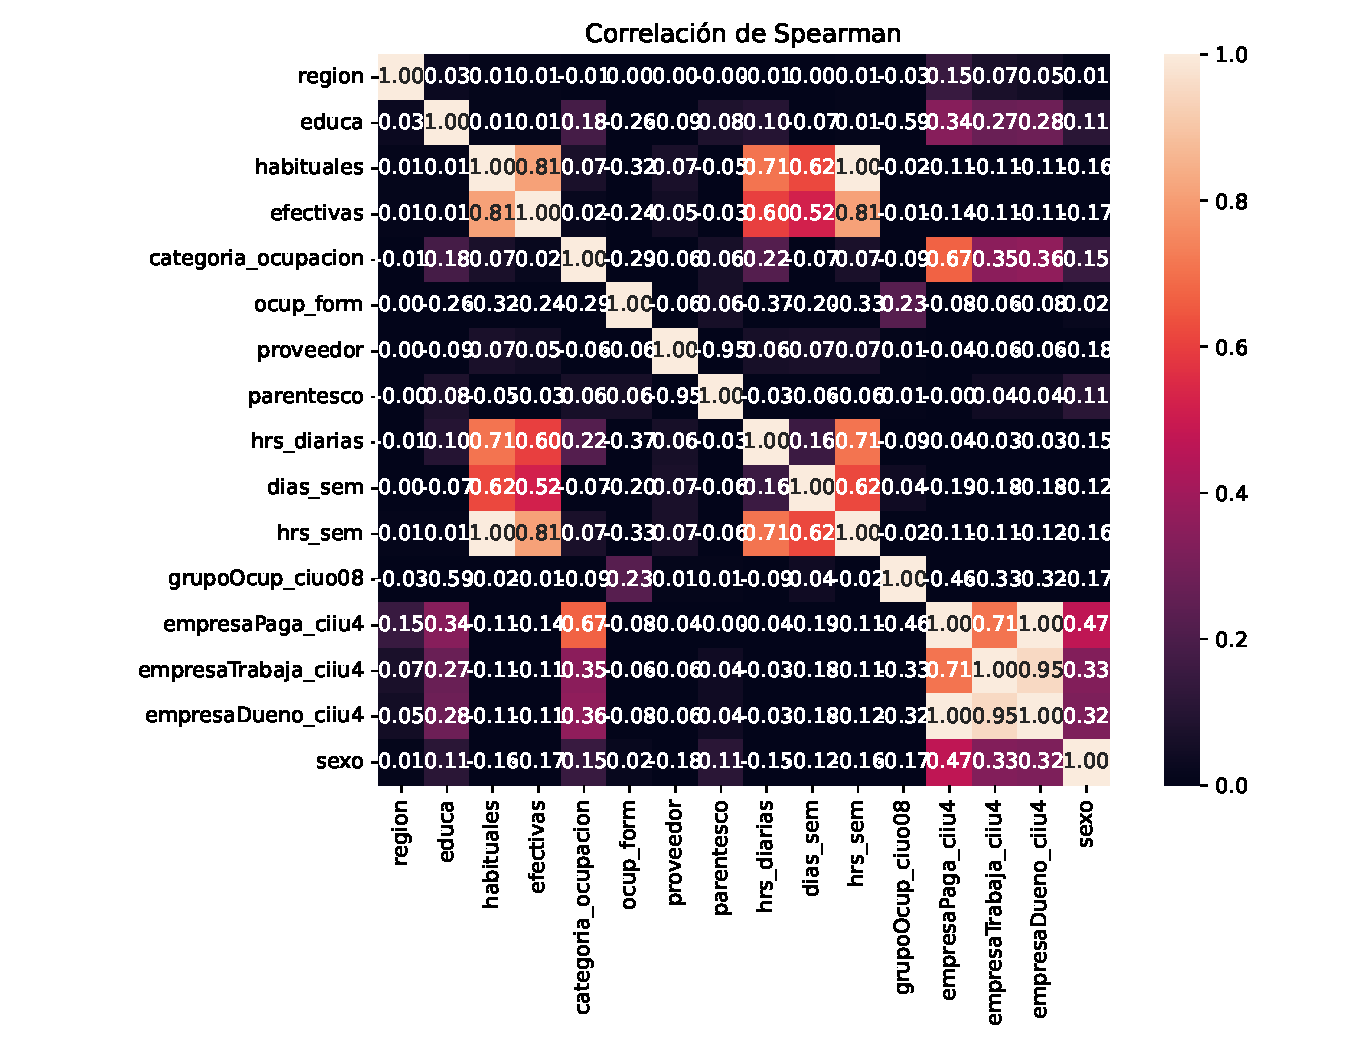
\includegraphics[width=\textwidth]{visualizaciones/finales/CorrelacionesENE2022.pdf}
		\caption{ENE 2022}
		\label{8a} 
	\end{subfigure}
	\hfill
	\begin{subfigure}[b]{0.49\textwidth}
		\centering
		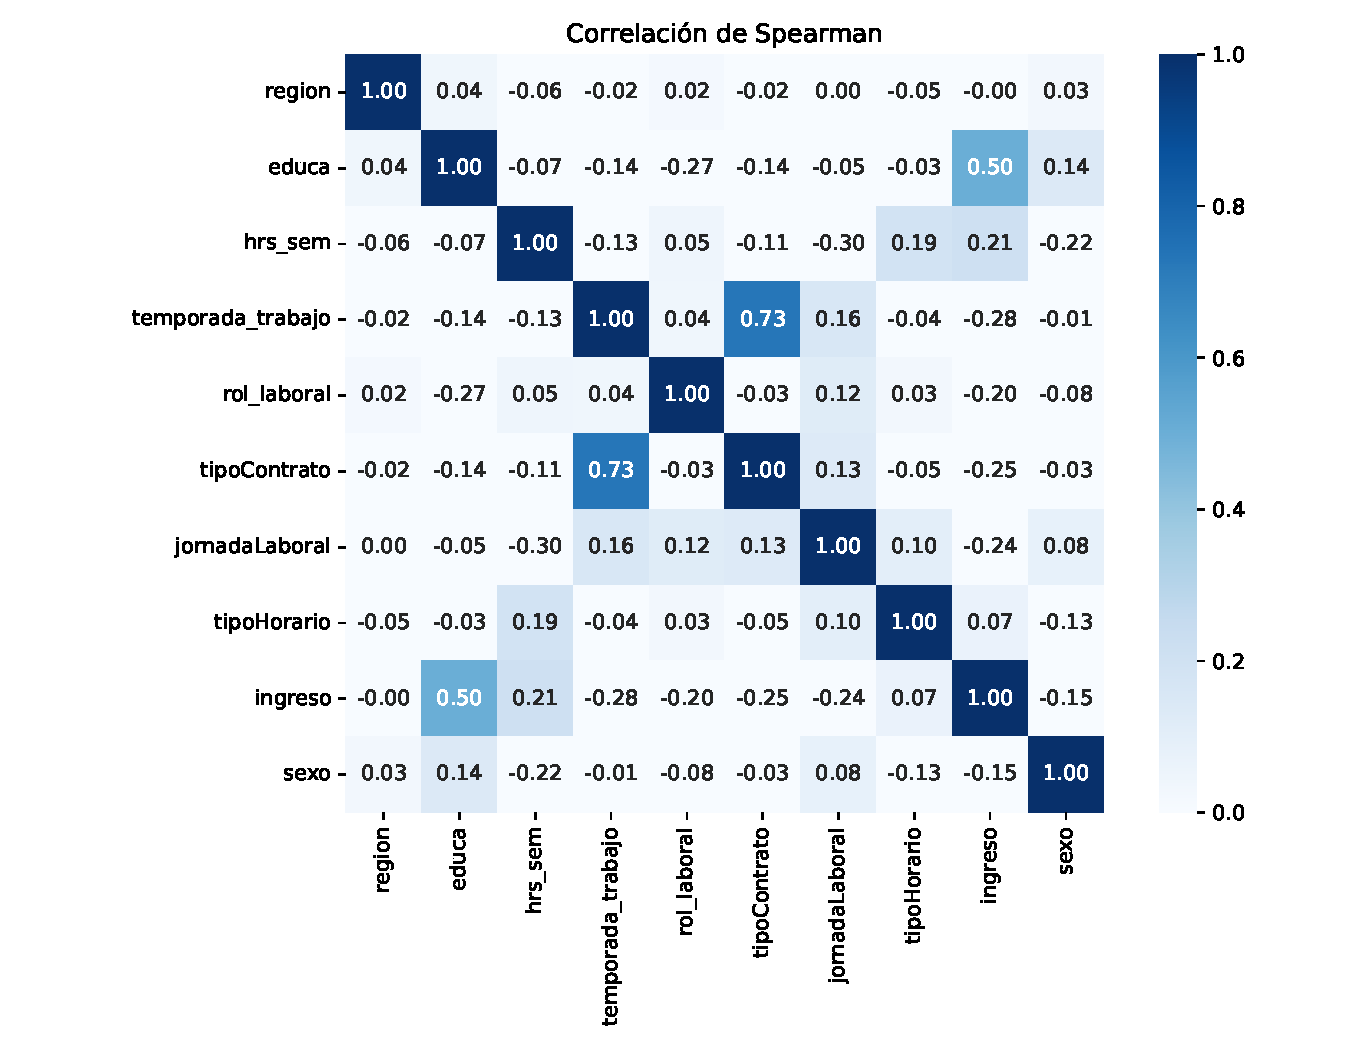
\includegraphics[width=\textwidth]{visualizaciones/finales/CorrelacionesCASEN2022.pdf}
		\caption{CASEN 2022}
		\label{8b}
	\end{subfigure}
	\caption{Correlación de Spearman entre variables en ENE y CASEN 2022}
	\label{08fig}
\end{figure}

\FloatBarrier

Como se observa en la Figura \ref{08fig} realizó correlación de Spearman en ambas encuestas para buscar patrones que permitan hallar una respuesta al problema de investigación. Principalmente se buscan variables laborales que sean capaces de tener una alta relación con el sexo. Sin embargo, lo que se observa son correlaciones muy bajas, donde la mayor relación la encontramos en la Figura \ref{8a}, viendo una máxima de 0.47 y una mínima de 0.32 con las variables de correspondientes a la rama de actividad económica (CIIU-4) de las empresas relacionadas a cada individuo, lo cual ya habíamos visualizado en la Figura \ref{4b} con el modelo de Random Forest.

\FloatBarrier

\begin{figure}[htbp]
	\centering
	\begin{subfigure}[b]{0.49\textwidth}
		\centering
		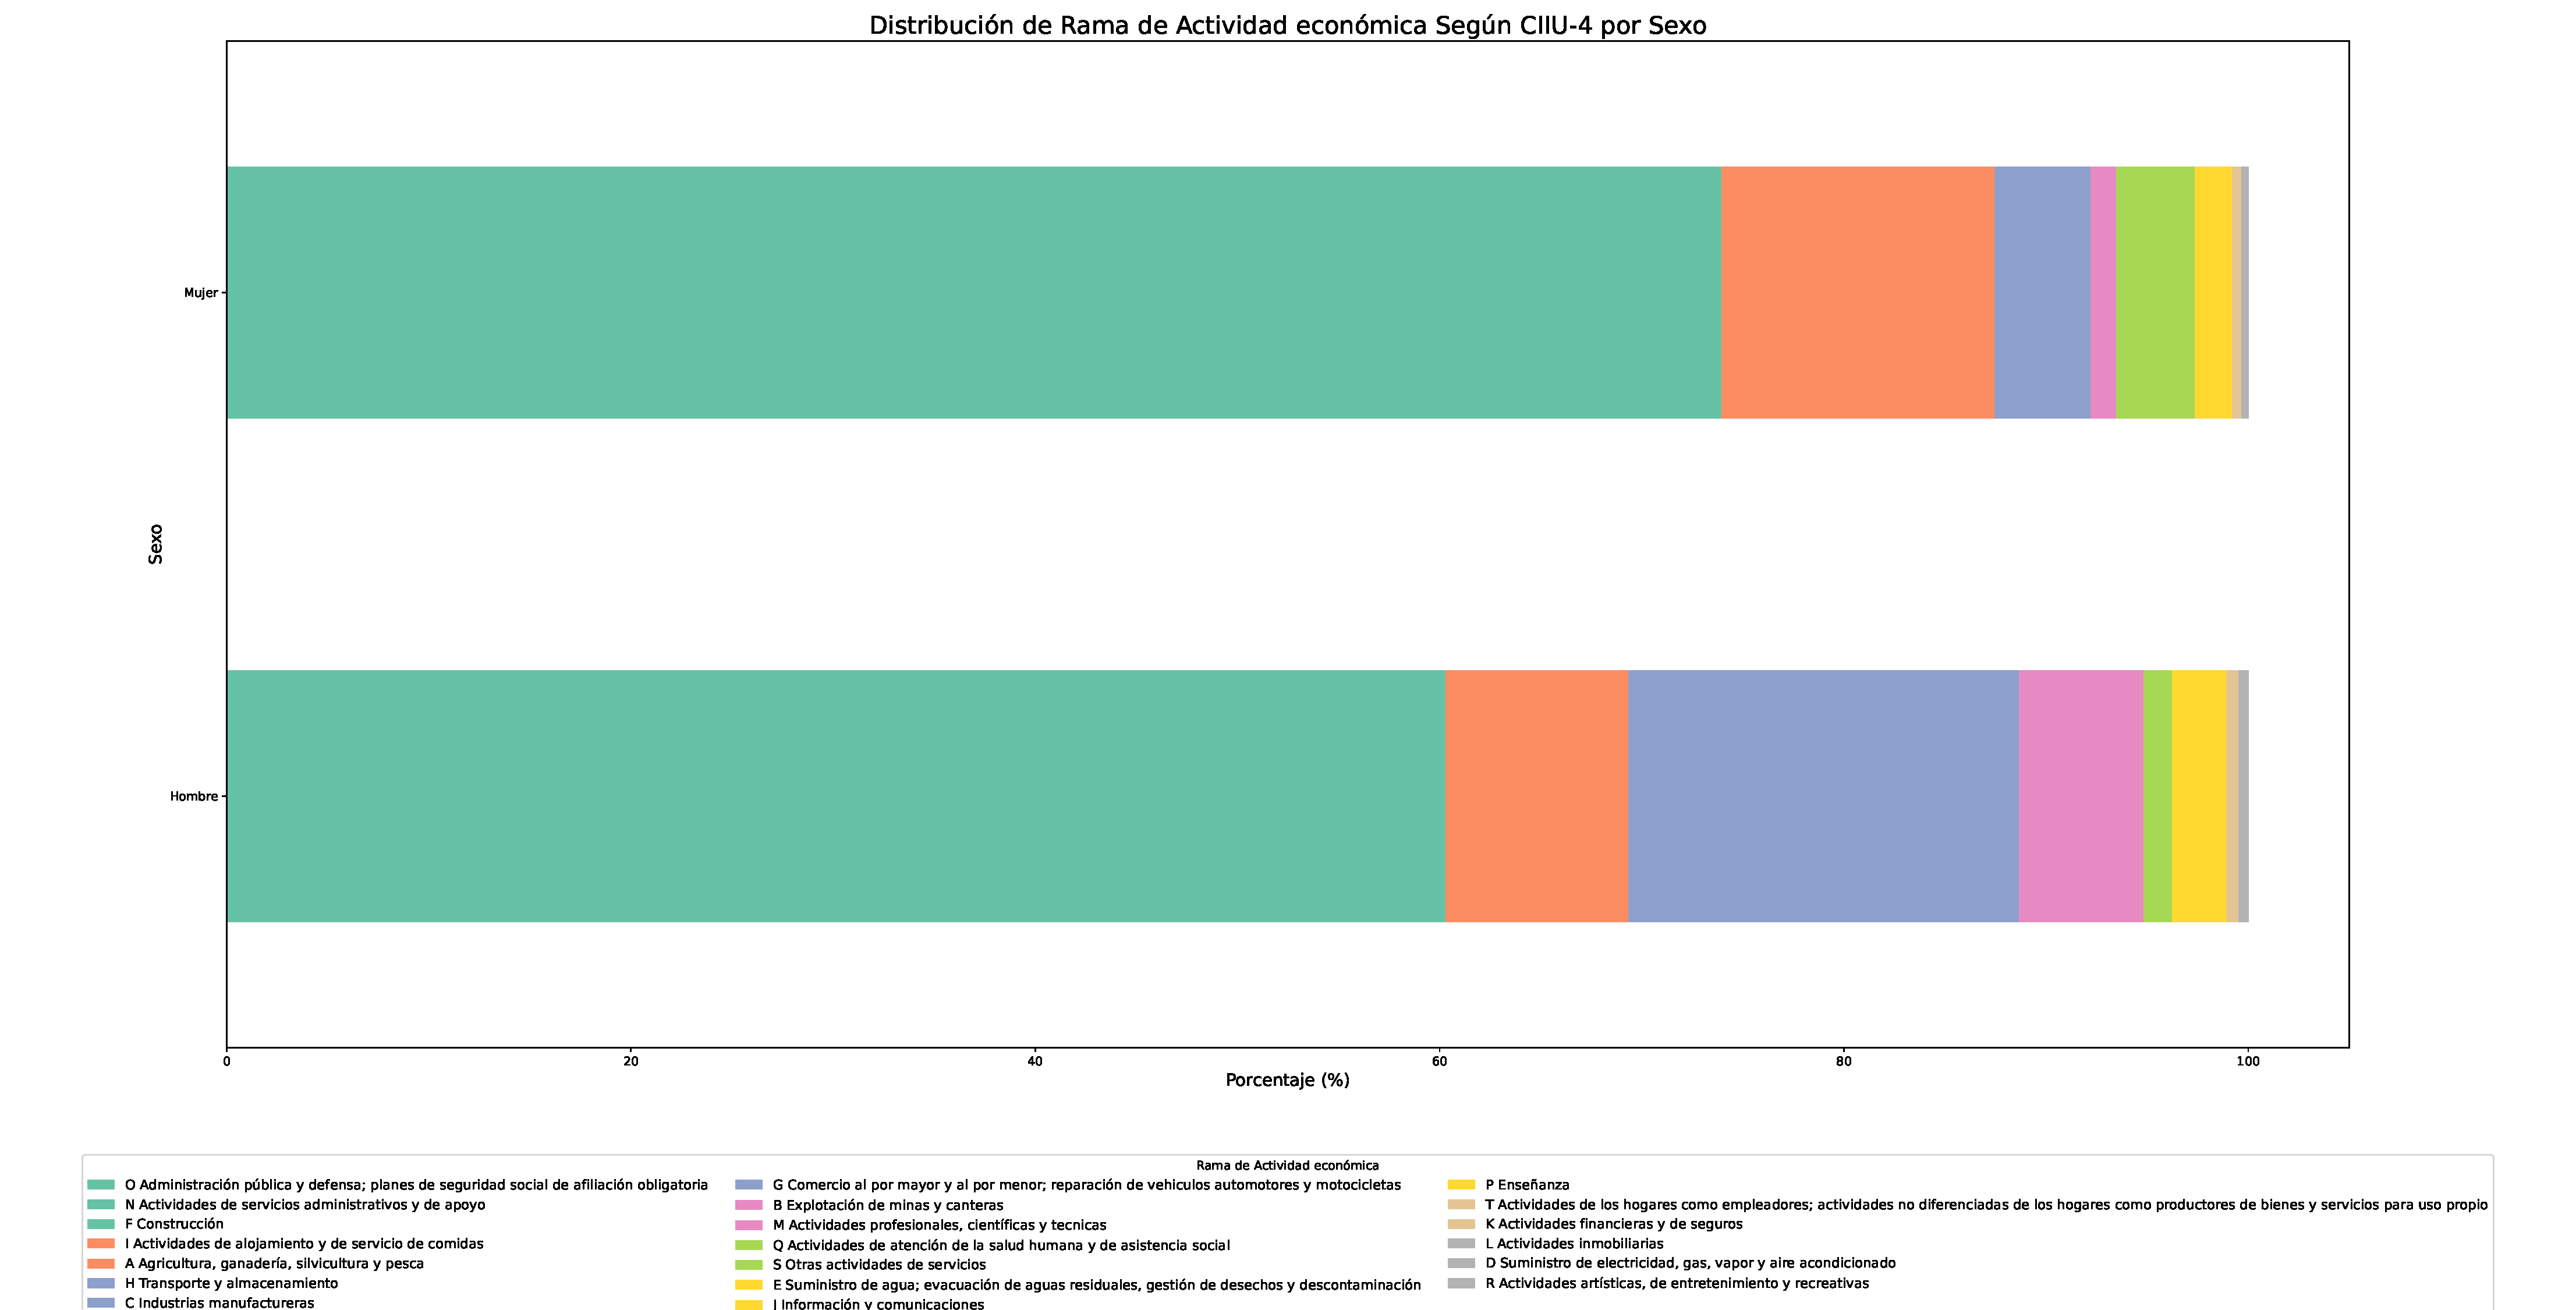
\includegraphics[width=\textwidth]{visualizaciones/finales/areaLabCIIU4_SexoENE2022.pdf}
		\caption{Rama de Actividad económica por CIIU-4.}
		\label{9a} 
	\end{subfigure}
	\hfill
	\begin{subfigure}[b]{0.49\textwidth}
		\centering
		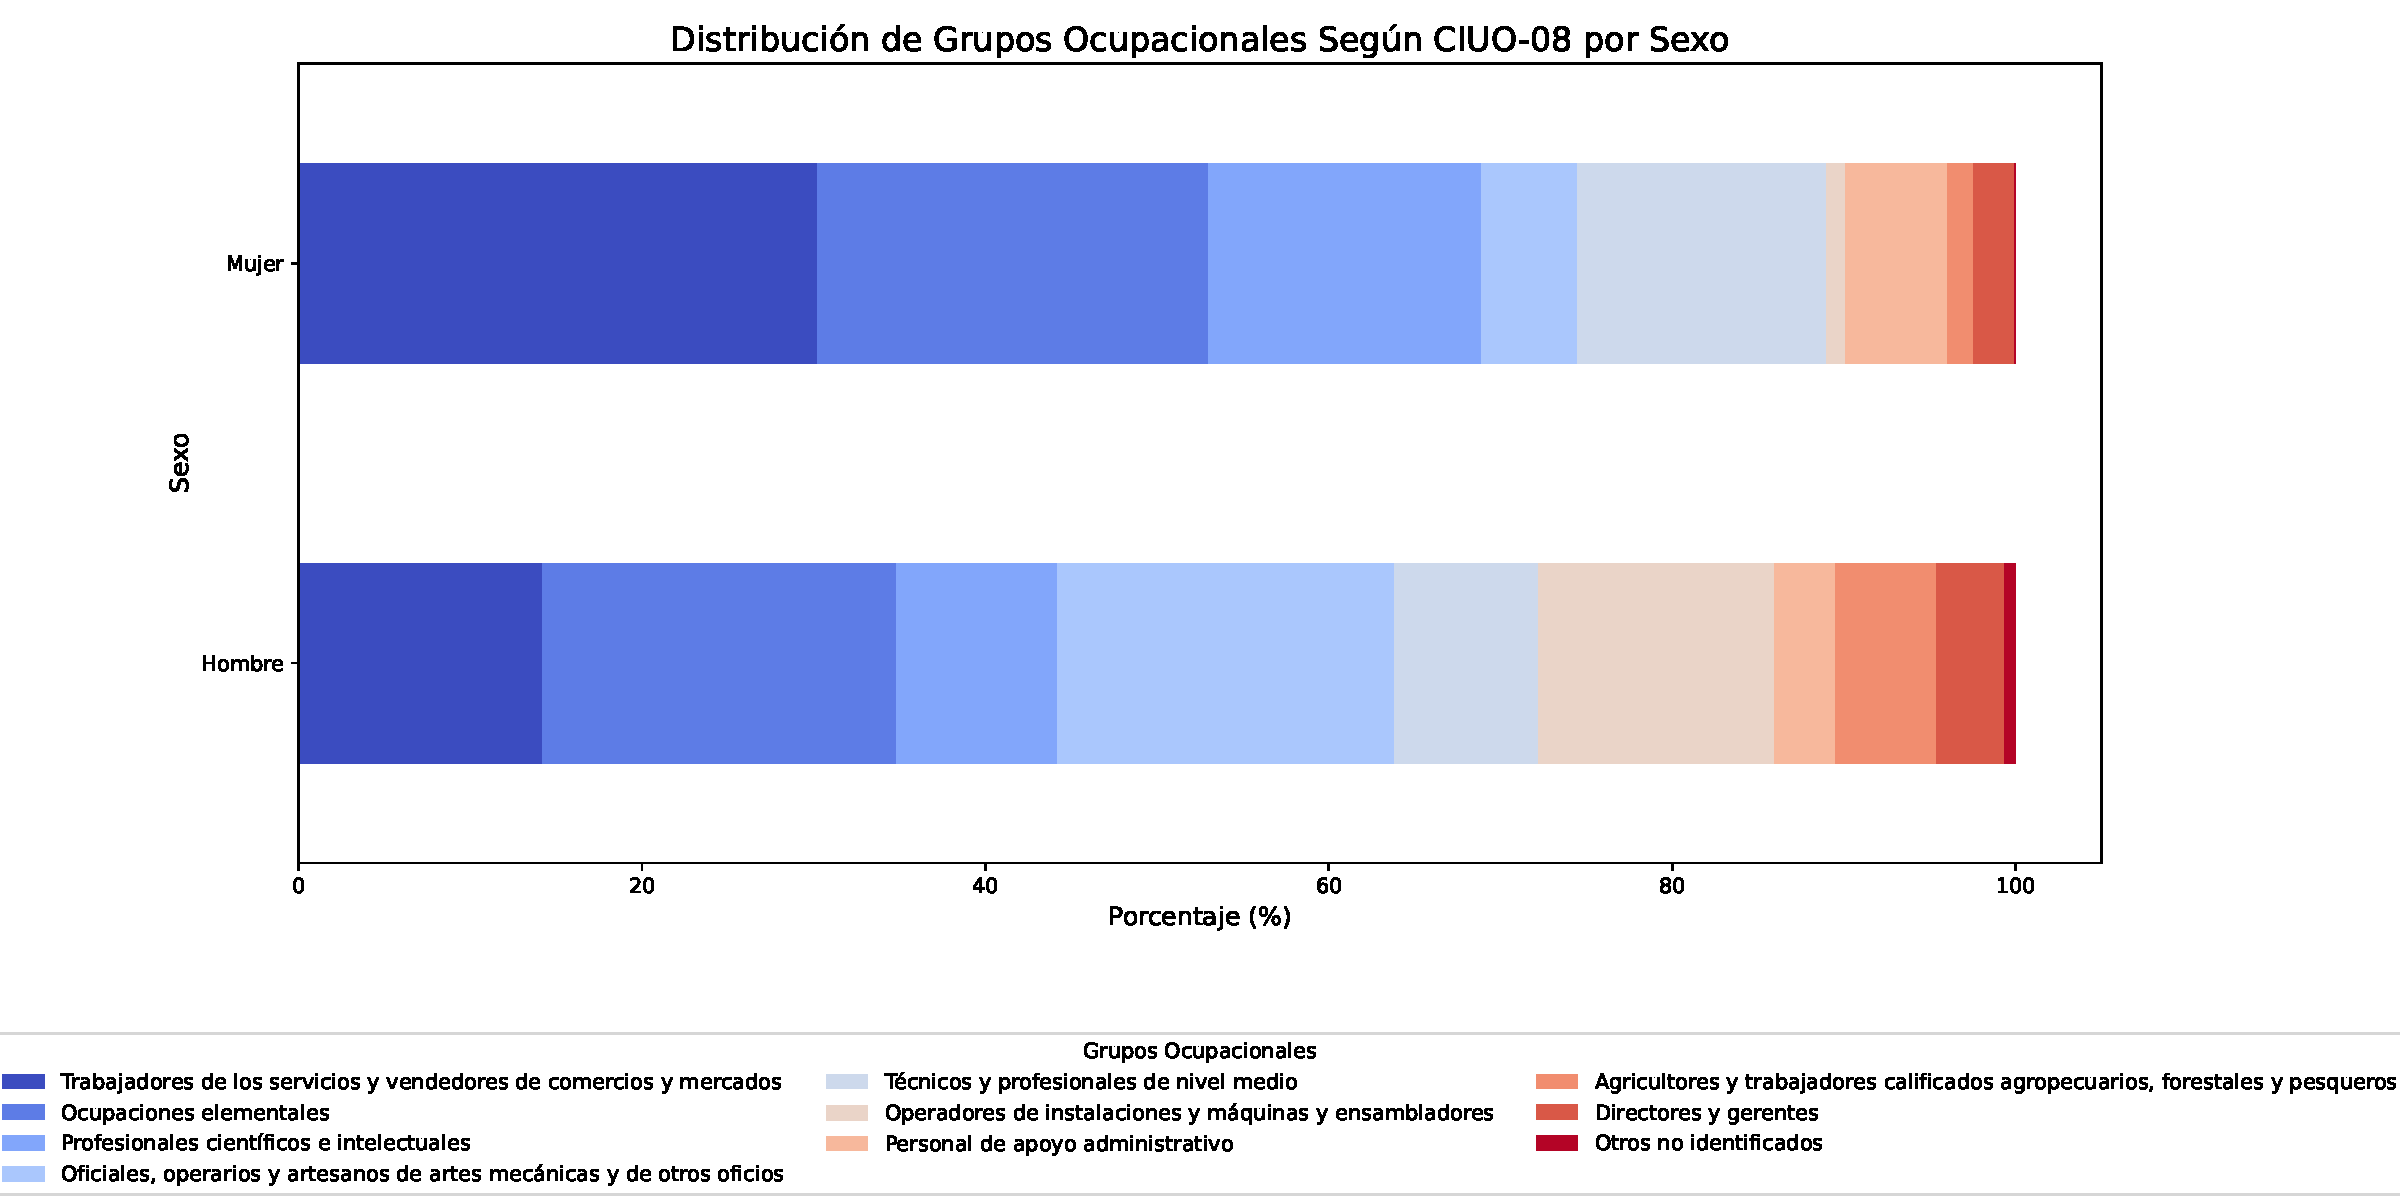
\includegraphics[width=\textwidth]{visualizaciones/finales/areaLabCIUO08_SexoENE2022.pdf}
		\caption{Grupos Ocupacionales por CIUO-08.}
		\label{9b}
	\end{subfigure}
	\caption{Distribución de áreas laborales por sexo. Elaborado en base a ENE 2022.}
	\label{09fig}
\end{figure}

\FloatBarrier

Analizando ahora las variables correspondientes a Rama de Actividad Económica (empresa que paga al trabajador) (CIIU-4), se osberva en la Figura \ref{9a} que existe una tendencia a cierto rubro de empresas, que incluyen el administración pública, actividades de servicios administrativos y construcción. Donde las mujeres tienen un porcentaje importante respecto a su total al igual que los hombres. Como segundo lugar, están los rubros de actividades de alojamiento y servicios de comida con agricultura, ganadería, silvicultura y pesca en el caso de las mujeres y los rubros de transporte y almacenamiento, industrias manufactureras y comercio al por mayor y menor para los hombres. Representando las demás ramas alrededor del 10\%.

Por otro lado, en la Figura \ref{9b} correspondiente a la distribución según Grupo Ocupacional (CIUO-08), vemos a las mujeres más concentradas en grupos como trabajadores de servicios y vendedores de comercios y mercados, mientras que la mayoría de los hombres están centrados en ocupaciones elementales, el cual es el segundo puesto del género femenino según la gráfica, mientras que el segundo puesto de los hombres vendría siendo el de oficiales, operarios y artesanos de artes mecánicas y de otros oficios. Se logra apreciar una distribución más pareja dentro del espectro de grupos ocupacionales en los hombres, mientras que las mujeres están un poco más concentradas en ciertos rubros. Esto también se hace visible, pero en menor medida en la Figura \ref{9a}.

\FloatBarrier

\begin{figure}[htbp]
	\centering
	\begin{subfigure}[b]{0.49\textwidth}
		\centering
		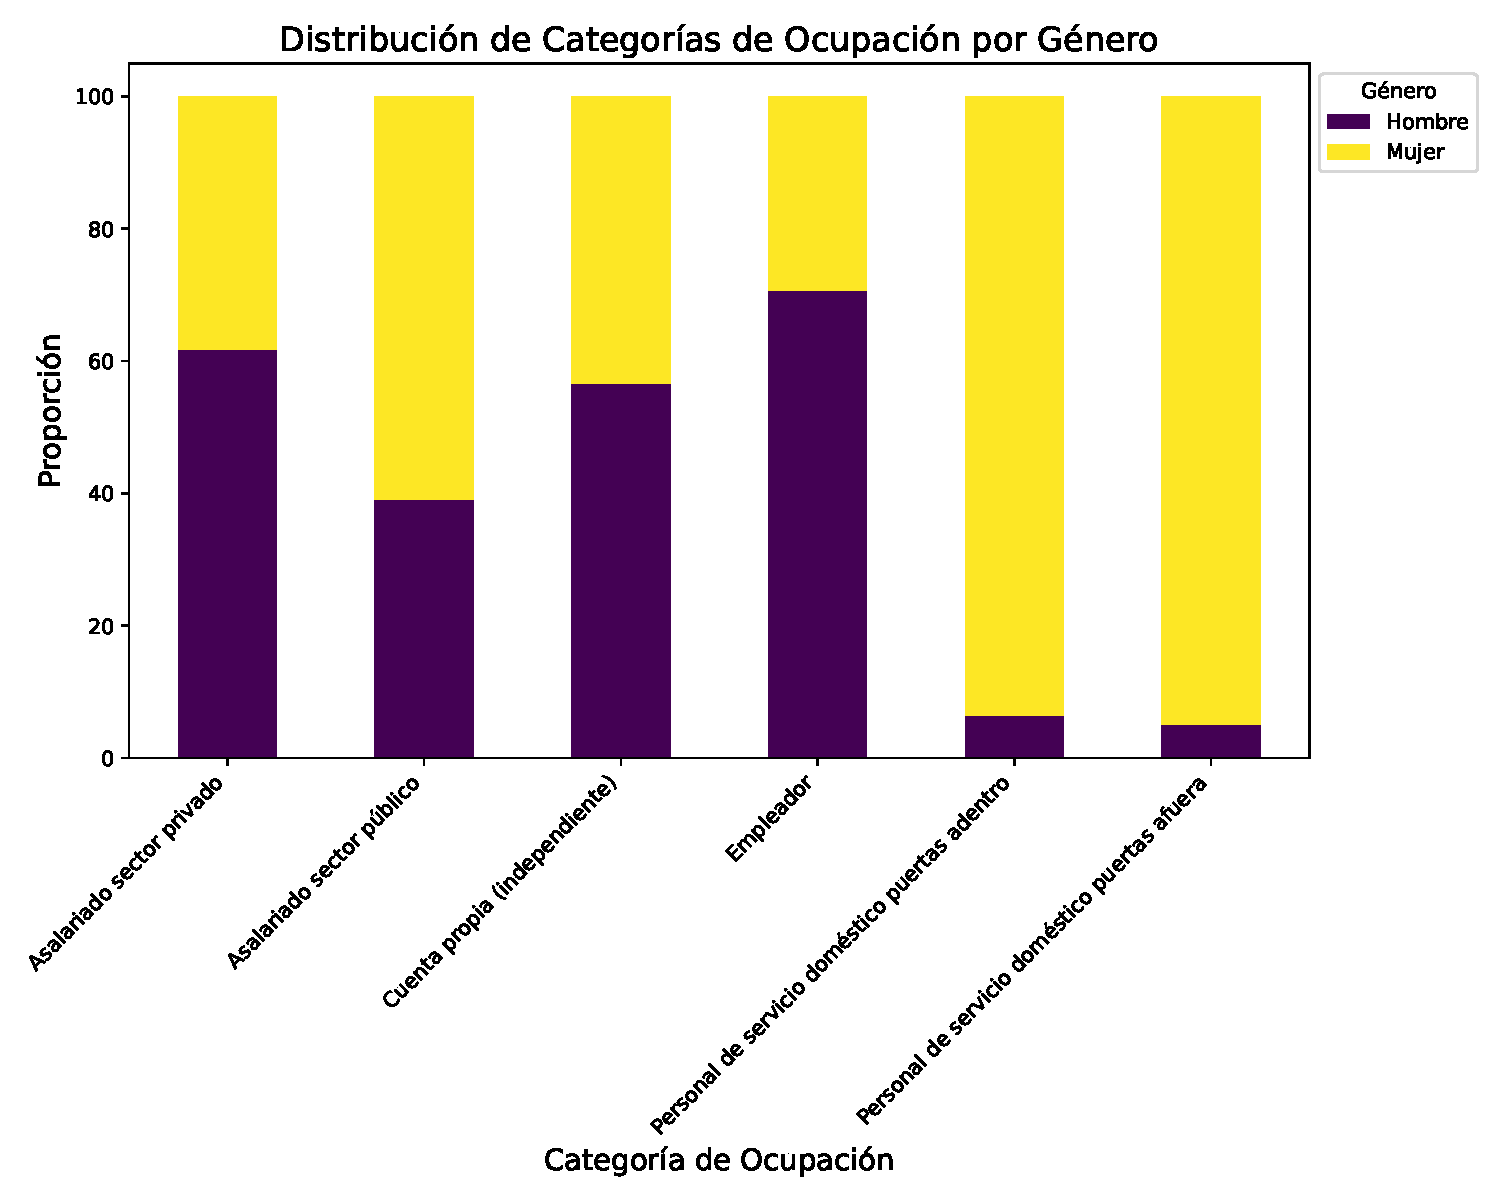
\includegraphics[width=\textwidth]{visualizaciones/finales/categoria_ocupacion_generoENE2022.pdf}
		\caption{Categoría de ocupación por género.}
		\label{10a} 
	\end{subfigure}
	\hfill
	\begin{subfigure}[b]{0.49\textwidth}
		\centering
		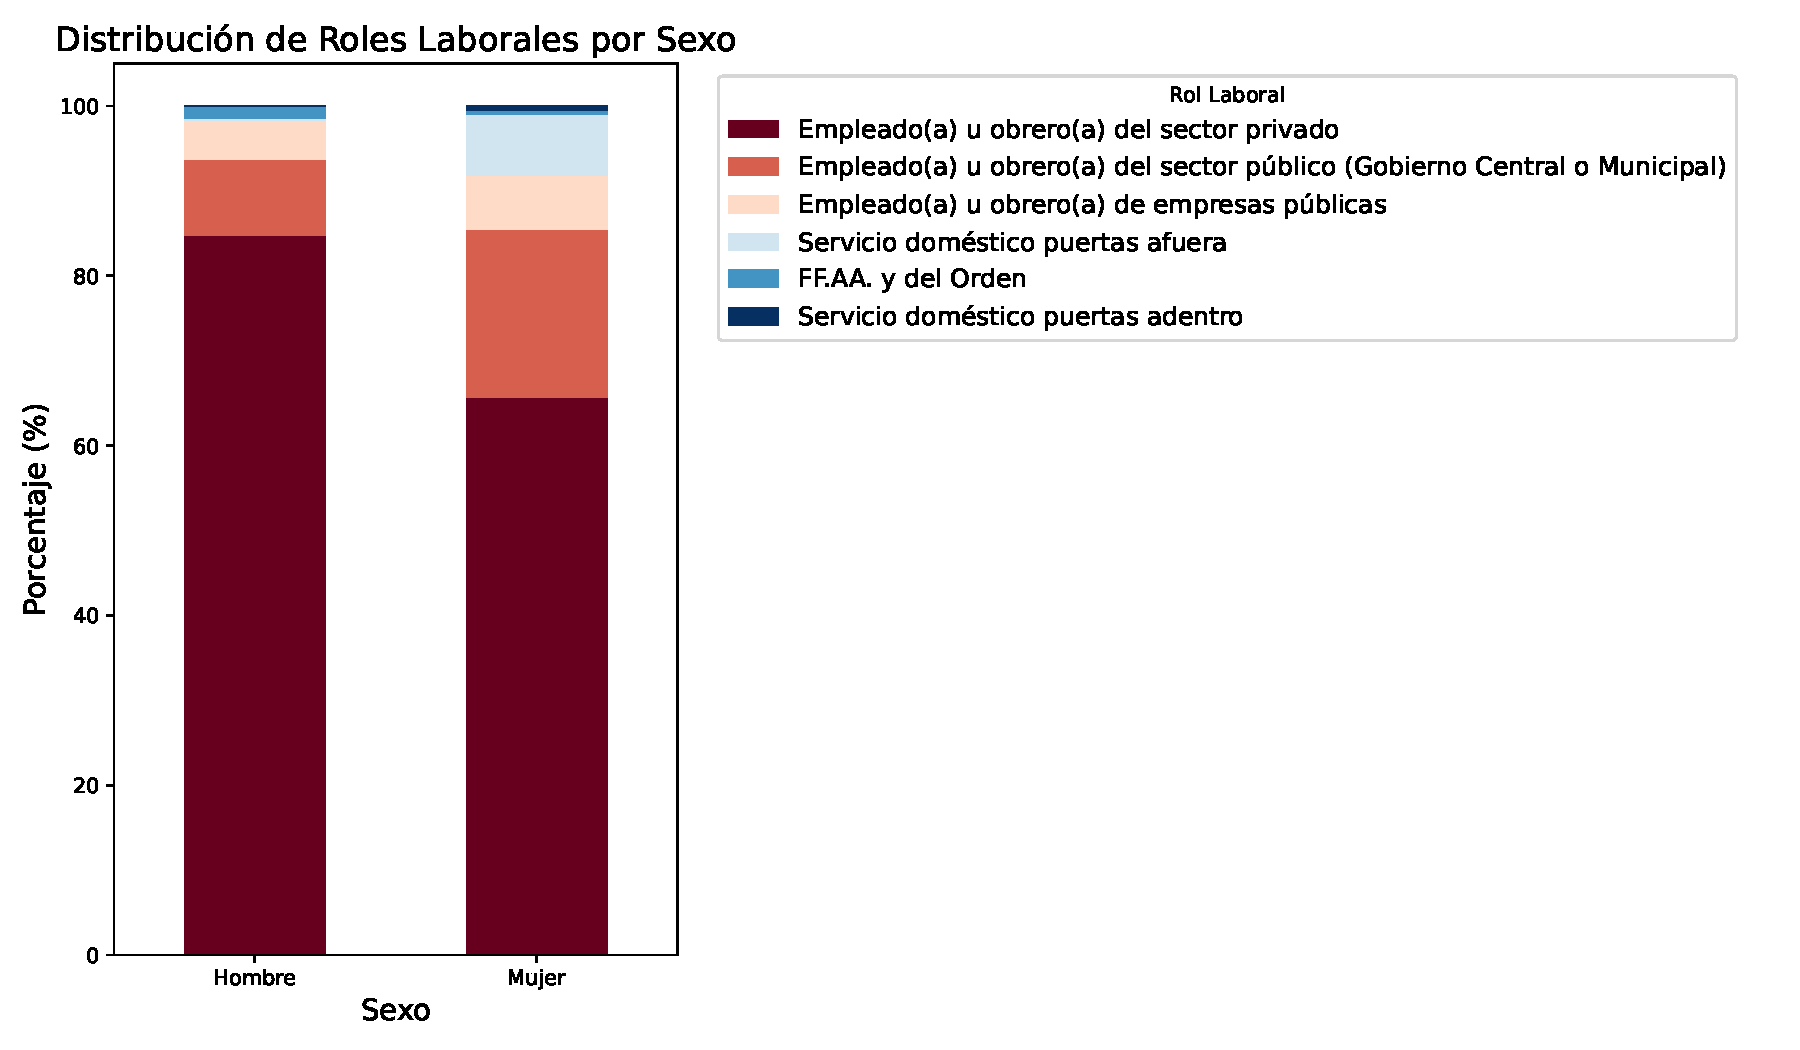
\includegraphics[width=\textwidth]{visualizaciones/finales/RolesLaboralesSexoCASEN2022.pdf}
		\caption{Roles laborales por género.}
		\label{10b}
	\end{subfigure}
	\caption{Distribución de Categoría de ocupación y Roles laborales por género. Elaborados en base a  en base a ENE y CASEN 2022 respectivamente.}
	\label{10fig}
\end{figure}

\FloatBarrier

Analizando la Figura \ref{10a} observamos que de las diferentes categorías de ocupación los hombres tienen mayor porcentaje en: 

\begin{itemize}
	\item Asalariado sector privado
	\item Cuenta propia (independiente)
	\item Empleador
\end{itemize}

Mientras que las mujeres tienen un mayor porcentaje en las categorías de:

\begin{itemize}
	\item Asalariado sector público
	\item Personal de servicio doméstico puertas adentro
	\item Personal de servicio doméstico puertas afuera
\end{itemize}

Por otra parte, en la Figura \ref{10b}, vemos que en cuanto a roles laborales por género, vemos que los hombres concentran más del 80\% en solo el rol de empleado u obrero del sector privado y sobrepasa el 90\% sumándole el rol de empleado u obrero del sector público. Mientras que las mujeres sobrepasan el 60\% como empleadas del sector privado, luego el 80\% como empleadas del sector público y ya pasan el 90\% como empleadas de empresas públicas. Es decir su concentración es un poco más distribuida que la de los hombres en este caso.

\FloatBarrier

\begin{figure}[htbp]
	\centering
	\begin{subfigure}[b]{0.49\textwidth}
		\centering
		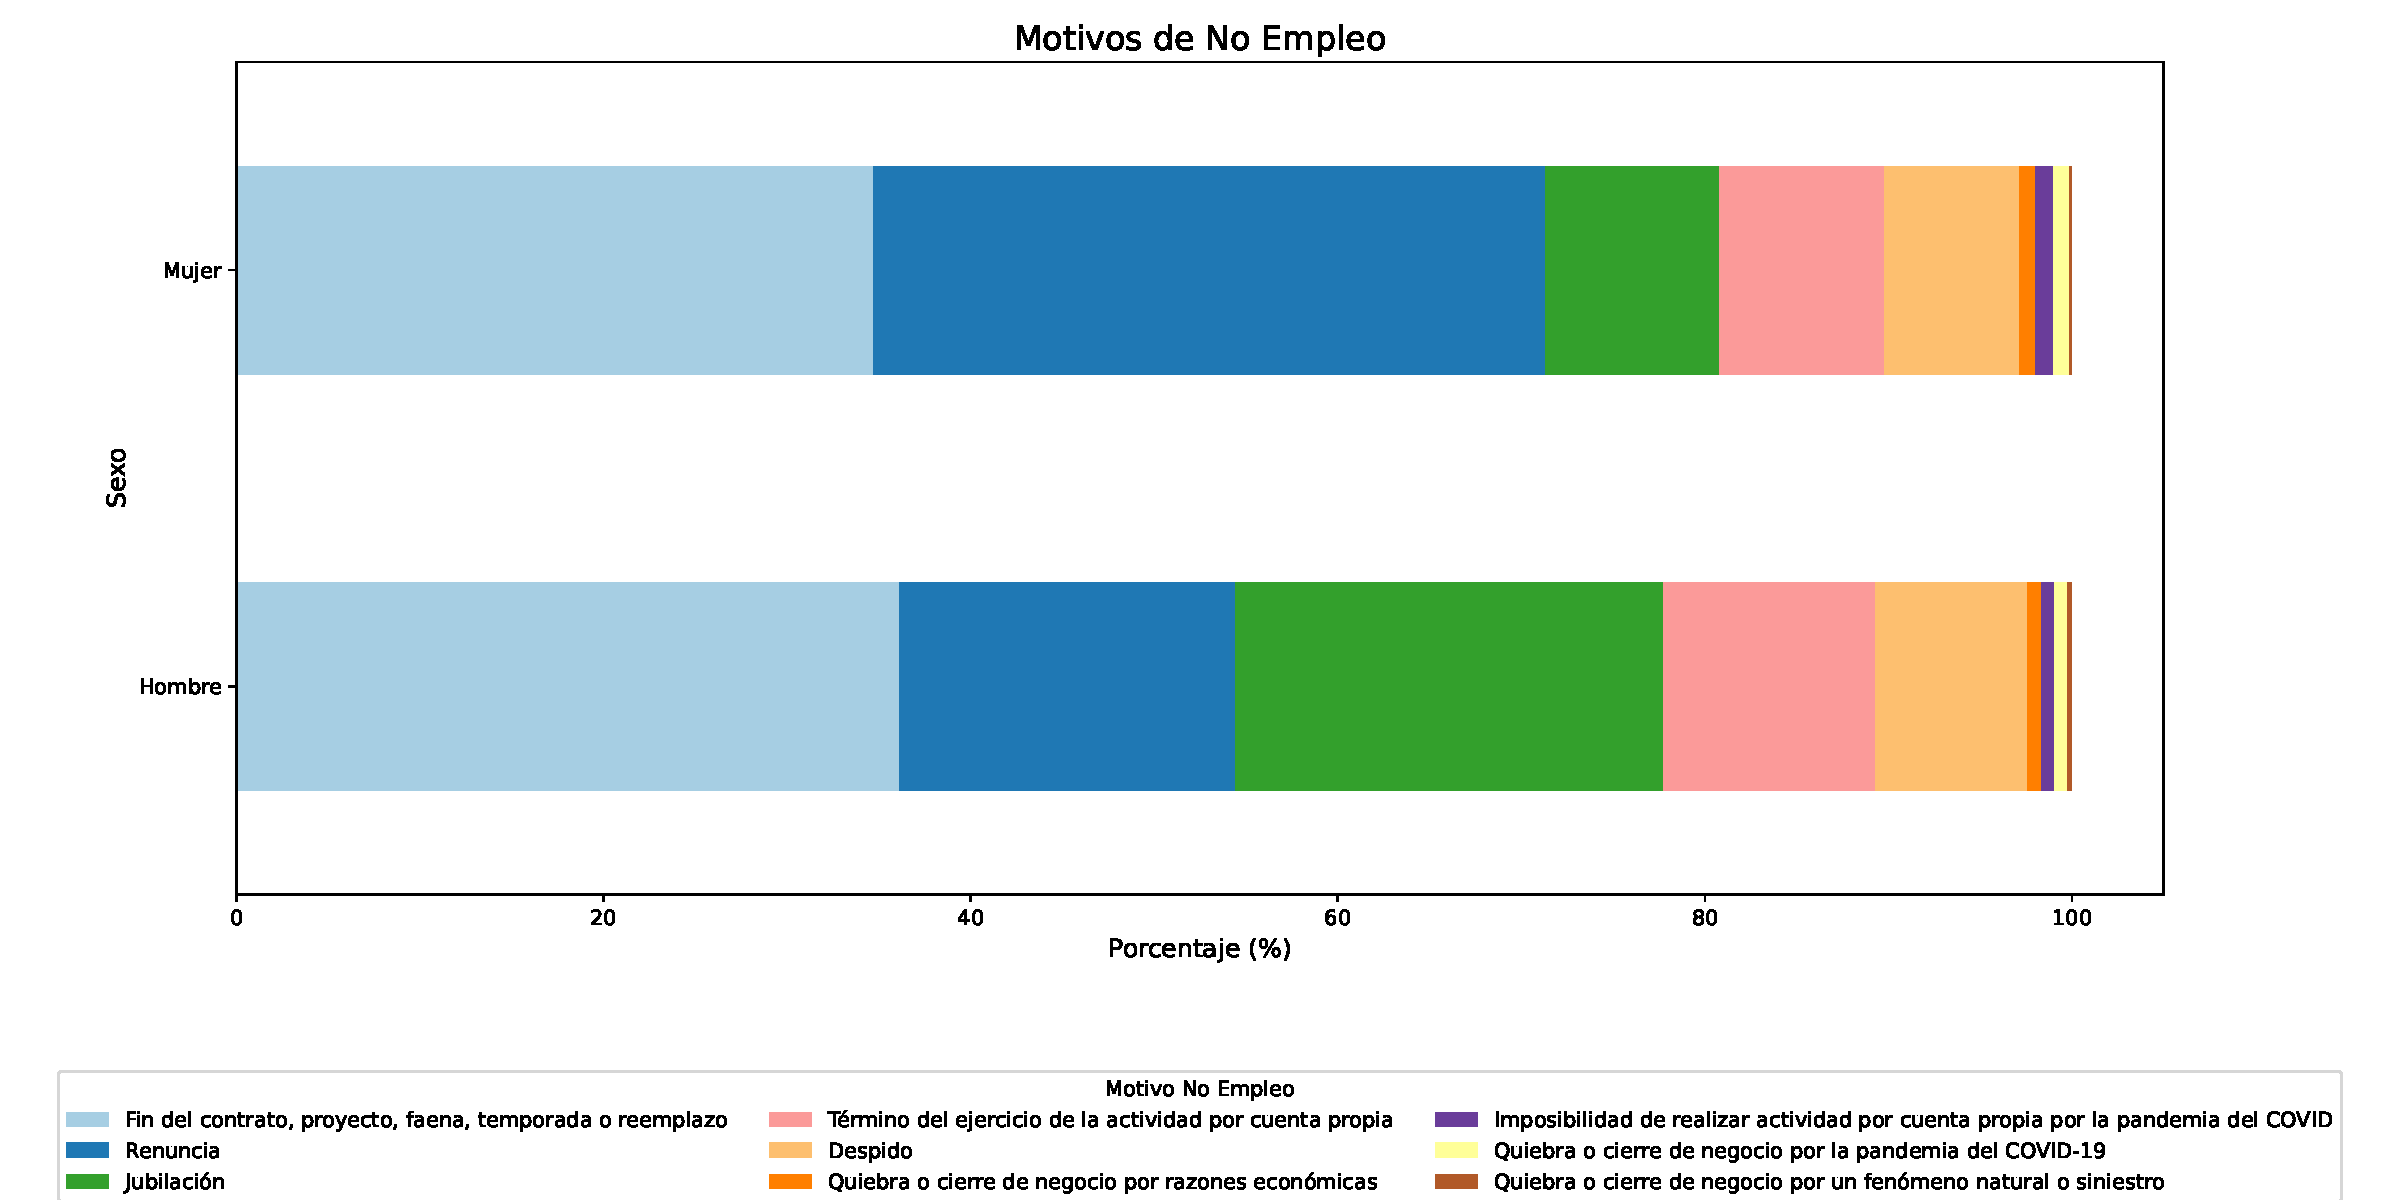
\includegraphics[width=\textwidth]{visualizaciones/finales/MotivoNoEmpleoENE2022.pdf}
		\caption{Motivos de No Empleo.}
		\label{11a} 
	\end{subfigure}
	\hfill
	\begin{subfigure}[b]{0.49\textwidth}
		\centering
		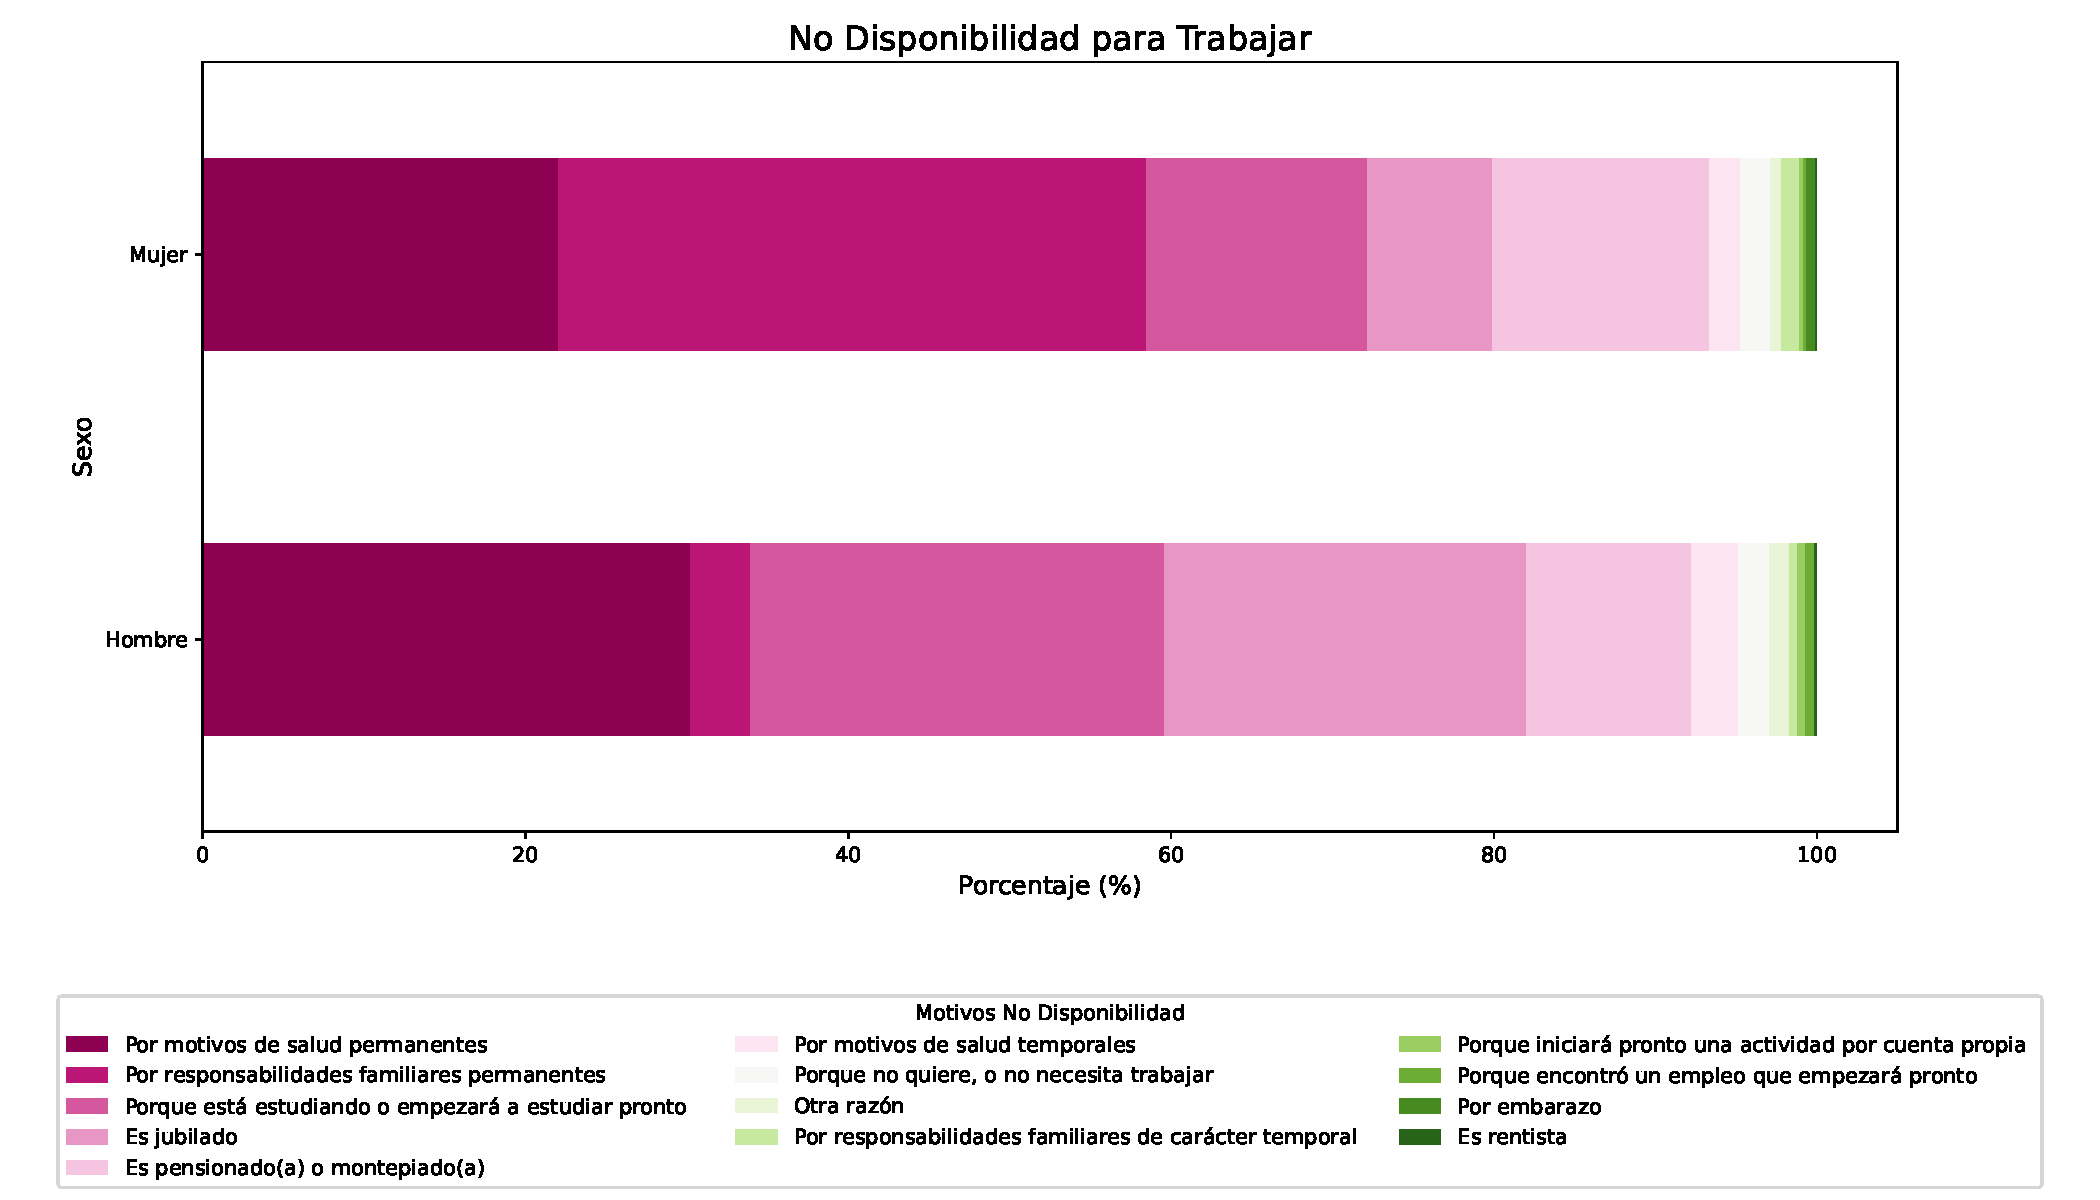
\includegraphics[width=\textwidth]{visualizaciones/finales/NoDisponibilidadENE2022.pdf}
		\caption{Motivos de No Disponibilidad para trabajar.}
		\label{11b}
	\end{subfigure}
	\caption{Razones por los que los encuestados no tienen empleo o no se encuentran disponibles para trabajar. Elaborado en base a ENE 2022.}
	\label{11fig}
\end{figure}

\FloatBarrier

Cuando se analizan los motivos de no empleo que muestra la Figura \ref{11a} vemos que en el caso de las mujeres, un gran porcentaje no tiene empleo porque renuncia a su trabajo, lo cual es muy llamativo, ya que representa aprox un 30\% del total, seguido por el fin de contrato, término de reemplazo o buena temporada. Asimismo, los hombres sin empleo tienen por motivo principal el fin de contrato, buena temporada o reemplazo. Le sigue la jubilación y en tercer lugar se encuentra la renuncia como motivo de no empleo, concentrando aprox un 15\%.

En cuanto a la no disponibilidad para trabajar de la Figura \ref{11b}llama la atención que el motivo principal de las mujeres es uno de los menos indicados por los hombres, siendoe este las responsabilidades familiares permanentes con aprox 35\% de los casos. Por otro lado, los hombres tienen como causa principal los motivos de salud permanentes con cerca de un 25\%, seguido de la jubilación con más o menos el mismo porcentaje.

Lo anterior indicaría que las mujeres principalmente cumplen con labores domésticas dentro de su rol social. Responsabilidad familiar permanente podría indicar el cuidado de un hijo o familiar enfermo que requiera cuidados. Además junto con las categorías de ocupación presentadas en la Figura \ref{10a}, se puede ligar una parte de la brecha salarial debido a que las mujeres realizan principalmente trabajo doméstico y reproductivo, el cual puede ser o no remunerado. 

Las proporciones de la Figura \ref{11a} indicarían que los hombres no llevan a cabo la reproducción social que si hacen las mujeres, pudiendo esto afectar la inserción laboral de estas. ``Si la sociedad norteamericana reconociese el trabajo doméstico y la crianza de los 
hijos como trabajo productivo cuantificable en los presupuestos económicos nacionales [...] la recepción de ayudas sociales no implicaría dependencia.'' \citep{Federici2013}

\FloatBarrier

\begin{figure}[htbp]
	\centering
	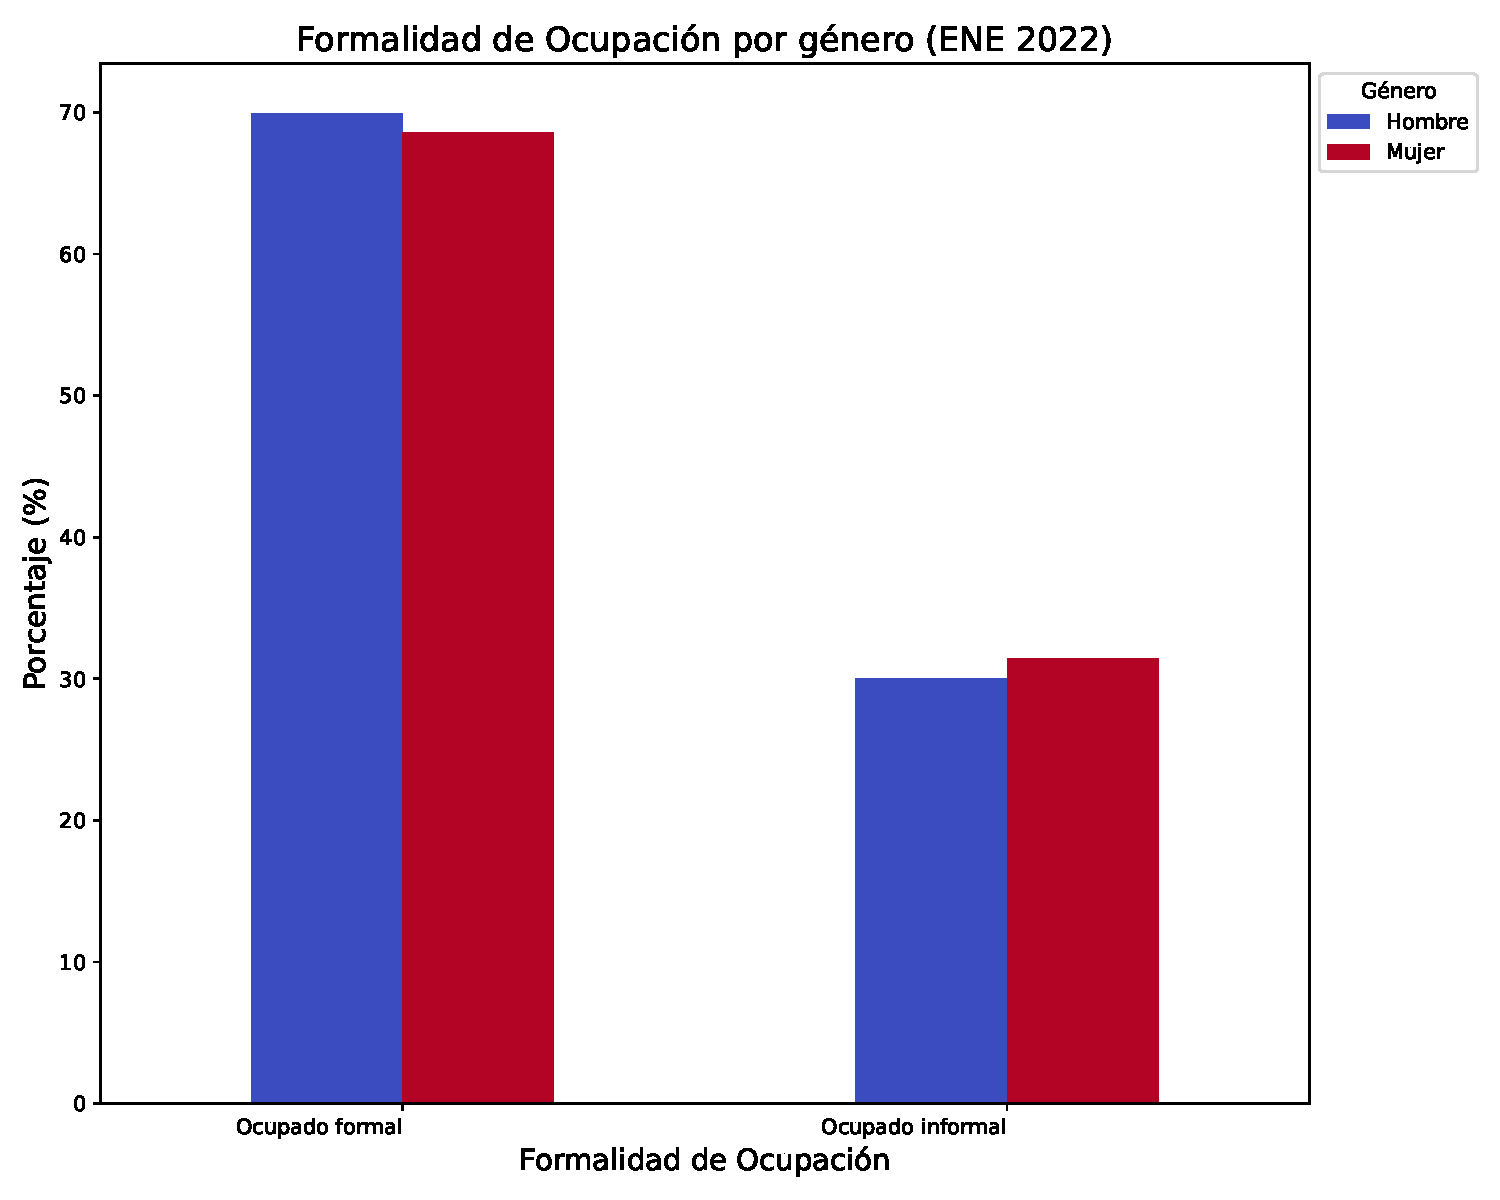
\includegraphics[width=0.65\textwidth]{visualizaciones/finales/FormalidadOcupacionENE2022.pdf}
	\caption{Formalidad de ocupación por sexo. Elaborado en base a ENE 2022.}
	\label{12fig} 
\end{figure}

\FloatBarrier

\begin{table}[htbp]
	\centering
	
	\begin{tabular}{|c|c|c|c|c|c|}
		\hline
		\multicolumn{3}{|c|}{\textbf{BuscarTrabajo}} & \multicolumn{3}{c|}{\textbf{Busca4semanas}} \\
		\hline
		\textbf{Sexo} & \textbf{Sí (1)} & \textbf{No (0)} & \textbf{Sexo} & \textbf{Sí (1)} & \textbf{No (0)} \\
		\hline
		Mujer & 4485 & 68892 & Mujer & 4507 & 68766 \\
		Hombre & 5156 & 57498 & Hombre & 5180 & 57288 \\
		\hline
		\textbf{Total} & 9641 & 126390 & \textbf{Total} & 9687 & 126054 \\
		\hline
	\end{tabular}
	\caption{Distribución por Sexo para las Variables ``BuscarTrabajo'' y ``Busca4semanas''(últimas 4). Elaborado en base a ENE 2022.}
	\label{tab:distribucion_sexo_2}
\end{table}

\FloatBarrier

Evaluando la Figura \ref{12fig} no se aprecia mayor diferencia entre hombres y mujeres respecto a la formalidad de su ocupación, casi un 70\% en ambos son ocupados formales, un poco menos en el caso de las mujeres y sucede a la inversa en el caso de ocupación informal, aproximadamente un 30\% de ambos casos, teniendo un poco más de porcentaje las mujeres, pero por lo general, están bastante parejos en este aspecto.

Por otro lado, se observa en el Cuadro \ref{tab:distribucion_sexo_2} que las mujeres buscan menos trabajo que los hombres, a pesar de tener mayor cantidad desempleada. Lo cual podría coincidir si lo juntamos con que aprox el 30\% no trabaja por responsabilidades familiares permanentes, pudiendo nuevamente asociar esto con el trabajo reproductivo y doméstico.

\FloatBarrier

\begin{table}[htbp]
	\centering
	\resizebox{\textwidth}{!}{
		\begin{tabular}{|c|c|c|c|c|c|c|c|c|}
			\hline
			\multicolumn{4}{|c|}{\textbf{ENE 2022}} & \multicolumn{4}{c|}{\textbf{CASEN 2022}} \\
			\hline
			\multicolumn{2}{|c|}{\textbf{Mujeres}} & \multicolumn{2}{c|}{\textbf{Hombres}} & \multicolumn{2}{c|}{\textbf{Mujeres}} & \multicolumn{2}{c|}{\textbf{Hombres}} \\
			\hline
			\textbf{Estado} & \textbf{Porcentaje (\%)} & \textbf{Estado} & \textbf{Porcentaje (\%)} & \textbf{Estado} & \textbf{Porcentaje (\%)} & \textbf{Estado} & \textbf{Porcentaje (\%)} \\
			\hline
			Ocupadas & 43.4 & Ocupados & 64.33 & Ocupadas & 44.1 & Ocupados & 65.45 \\
			Desocupadas & 56.6 & Desocupados & 35.67 & Desocupadas & 55.9 & Desocupados & 34.55 \\
			\hline
			\multicolumn{4}{|c|}{\textbf{Distribución General (Ocupados)}} & \multicolumn{4}{c|}{\textbf{Distribución General (Ocupados)}} \\
			\hline
			\multicolumn{2}{|c|}{\textbf{Sexo}} & \multicolumn{2}{c|}{\textbf{Porcentaje (\%)}} & \multicolumn{2}{c|}{\textbf{Sexo}} & \multicolumn{2}{c|}{\textbf{Porcentaje (\%)}} \\
			\hline
			\multicolumn{2}{|c|}{Hombre} & \multicolumn{2}{c|}{55.86} & \multicolumn{2}{c|}{Hombre} & \multicolumn{2}{c|}{56.13} \\
			\multicolumn{2}{|c|}{Mujer} & \multicolumn{2}{c|}{44.14} & \multicolumn{2}{c|}{Mujer} & \multicolumn{2}{c|}{43.87} \\
			\hline
		\end{tabular}
	}
	\caption{Tasa de Ocupación y Desocupación de Hombres y Mujeres según ENE 2022 y CASEN 2022.}
	\label{tab:ocupacion_ene_casen}
\end{table}

\FloatBarrier

Cuando se analiza la tasa de ocupación en ambas encuestas, se hace evidente que las mujeres tienen tanto menor porcentaje de ocupación respecto a su género, como respecto al general ocupado tanto en la ENE como en CASEN, motivos claros a esto no hay. Sin embargo, se puede nuevamente ligar todo a lo ya visto en las gráficas y tablas anteriores. 

\FloatBarrier

\section{Conclusiones}

En este proyecto, se ha aborado el problema de la brecha salarial de género en Chile durante el año 2022. Para ello se realizaron análisis de las encuestas CASEN y ENE a través de Python y sus librerías. Los resultados obtenidos validan la hipótesis inicial, que planteaba que en promedio las mujeres ganan menos que los hombres incluso estando en similitud de condiciones laborales, lo cual es cierto. No existe una diferencia justificada por variables laborales que permita definir el porqué las mujeres reciben salarios inferiores a los hombres. 

El contraste entre ambos géneros no reflejaba la disparidad salarial encontrada. Si bien podría explicarse hasta cierto punto con la cantidad de horas (diarias/semanales), días a la semana trabajados, rama de actividad económica de la empresa y grupos ocupacionales, no hay cercanía alguna a dar respuesta al 100\% del problema. 

Hubo ciertas limitaciones como la calidad de los datos, ya que existían muchos valores nulos en las variables de relevancia para este proyecto. No obstante, se buscó constantemente minimizar al máximo cualquier inconveniente relacionado a la disminución de datos. Considero que esta temática no está del todo zanjada, aunque con los avances obtenidos, parece apuntar a que la brecha salarial de género surge directamente de una discriminación por este mismo a través del sueldo, realizando pagos inferiores a las mujeres sin mayor motivo.